\chapter{The \chips R\&D Project} %%%%%%%%%%%%%%%%%%%%%%%%%%%%%%%%%%%%%%%%%%%%%%%%%%%%%%%%%%%%%%%%
\label{chap:chips}

In pursuit of answers to the open questions presented in the previous chapter, neutrino
experiments are becoming increasingly, and possibly prohibitively, expensive and impractical. This
trend is particularly true of the next generation of long-baseline experiments, DUNE and
Hyper-Kamiokande, with cost estimates reaching billions of dollars and construction times of
greater than half a decade. It is also telling that the vast majority of global research effort
goes into just these two future projects, such is their complexity, cost, and lead time.

It is clear that for detectors to remain practical and affordable into the future, a novel design
strategy is highly desirable. This approach is especially the case if megaton scale detectors are
ever to become a reality. While instrumentation will continue to improve with time, the statistics
of low event counts will always limit neutrino experiments until vastly larger detectors can be
built. Therefore, R\&D efforts must focus on such detectors now, whilst also attempting to
complement the current and upcoming generation of experiments.

The \chips R\&D project~\cite{adamson2013} aims to develop novel strategies and technologies for
very large yet `cheap as chips' water Cherenkov detectors. Primarily aimed for deployment in long
baseline accelerator beam scenarios, \chips aims to lower the cost per kt of sensitive mass to
between \$200k-\$300k. For comparison, the Super-Kamiokande detector cost approximately \$4
million/kt to build. As physics sensitivity depends on more than just sensitive mass, this
comparison is not entirely rigorous; however, it highlights the scale of possible cost savings.

This chapter aims to describe the fundamental aspects of the \chips R\&D project in detail.
Firstly, the \chips concept will be outlined along with neutrino beam and Cherenkov detector
physics for context. The design, construction, deployment, and status of the \chipsfive prototype
detector will then follow. Finally, the Monte Carlo event generation and detector simulation
framework will be introduced to aid the discussion of work presented in later chapters of this
thesis.

\section{\chips concept} %%%%%%%%%%%%%%%%%%%%%%%%%%%%%%%%%%%%%%%%%%%%%%%%%%%%%%%%%%%%%%%%%%%%%%%%%
\label{sec:chips_concept} %%%%%%%%%%%%%%%%%%%%%%%%%%%%%%%%%%%%%%%%%%%%%%%%%%%%%%%%%%%%%%%%%%%%%%%%

The \chips concept is to deploy cylindrical water Cherenkov detector modules into deep bodies of
water on the Earth's surface such as lakes, reservoirs and flooded mine pits. Initially
constructed on land \chips detectors can be floated into position before being sunk. The water
above the sunken detector provides a modest overburden from cosmic rays, while the surrounding
water provides support for a lightweight detector structure. By removing the need for underground
excavation and expensive structural support, the cost of construction can be dramatically reduced.

Additionally, the common practice of building majority bespoke components is replaced by using
modern commercially available components wherever possible. The number of expensive elements, such
as photomultiplier tubes is also reduced by only considering multi-$\GeV$ accelerator beam
neutrino events, such that full high density and high coverage detector instrumentation is not
required.

Furthermore, \chips detectors are not only designed to be cheap but practical. Easy to build,
quick to deploy, and upgradable once operational, multiple detector modules can be flexibly
combined depending on available resources. When compared to DUNE and Hyper-Kamiokande both
requiring a large upfront budget and many years to construct, cheap \chips detector modules can be
deployed as needed in under a year by a relatively small team.

To date, \chips R\&D efforts have been based in the USA to exploit the NuMI beam before the end of
its lifetime. Plans are focused on the scaling of \chips detectors for the deployment of multiple
modules within the LBNF beam once operational. Collaborators from primarily University College
London, The University of Wisconsin Madison, and Nikhef are focused on multiple R\&D efforts,
outlined below, each aiming to prove the viability of a crucial component of the \chips concept.

\begin{itemize}
    \item \textbf{Detector construction:} Aiming to prove that the construction and deployment of
          \chips concept detector modules are possible. Two prototype detectors have so far been
          deployed. Firstly, the small \chipsm detector shown in Fig.~\ref{fig:chips_m}, deployed
          into a flooded mine pit in northern Minnesota during the summer of 2014~\cite{perch2015,
              pfutznerProto2017, pfutzner2017}. Secondly, the much larger \unit{5}{\mathrm{kt}}
          \chipsfive detector, deployed into the same pit during the summer of 2019 and detailed
          in Section.~\ref{sec:chips_detector}.

    \item \textbf{Water filtration:} Aiming to prove that adequate water purity can be achieved
          using cheap, commercially available filtration. Extensive studies have proven that by
          filtering water directly from bodies of water on the Earth's surface (including flooded
          mine pits), adequate photon attenuation lengths greater than \unit{50}{\mathrm{m}} are
          achievable~\cite{amat2017, campbell2020}.

    \item \textbf{Physics sensitivity:} Aiming to prove that \chips concept detectors (even the
          prototypes) can provide significant physics contributions alone or alongside the current
          and next generation of experiments. Single modules in the current NuMI beam (discussed
          in Section.~\ref{sec:chips_concept_beam}) and multiple modules in the future LBNF beam
          have been studied~\cite{pfutzner2017, adde2016, lang2015}.

    \item \textbf{Data acquisition:} Aiming to prove that a cheap data acquisition (DAQ) system
          using commercially available components and software is viable~\cite{eijk2018}. Outlined
          in Chapter.~\ref{chap:daq}, \chips implements a novel use of cheap single-board
          computers to collect photomultiplier tube data.

    \item \textbf{Event reconstruction and classification:} Aiming to prove that modern machine
          learning techniques can be successfully applied to large water Cherenkov concepts such
          as \chips. The primary contribution of this theis, detailed in Chapter.~\ref{chap:cvn},
          this work feeds directly into both physics sensitivity studies mentioned above and
          detector module optimisation studies.
\end{itemize}

\begin{figure} % CHIPS-M DIAGRAM %
    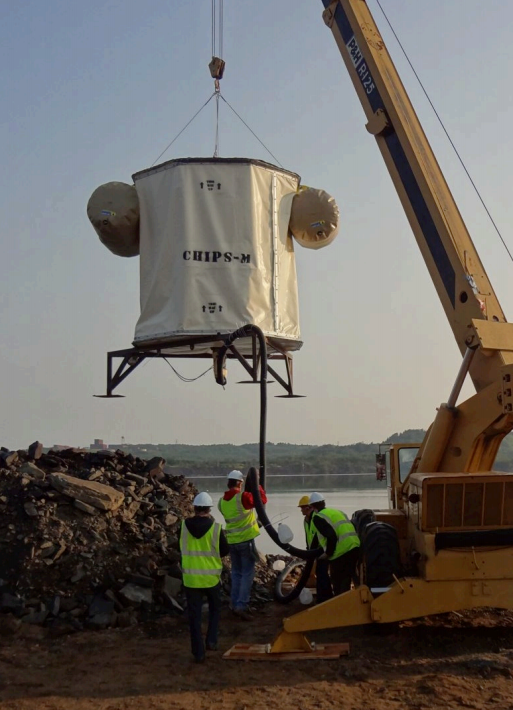
\includegraphics[width=0.6\textwidth]{diagrams/4-chips/chips_m.png}
    \caption[Picture of the \chipsm detector.]
    {Picture of the \unit{3.3}{\mathrm{m}} high \chipsm detector just before deployment. The
        temporary floatation bags are visibly attached to the top rim of the detector.
        Additionally, the umbilical cord carrying data, power, and filtered water is attached to
        the bottom of the detector.}
    \label{fig:chips_m}
\end{figure}

\subsection{The neutrino beam and off-axis alignment} %%%%%%%%%%%%%%%%%%%%%%%%%%%%%%%%%%%%%%%%%%%%
\label{sec:chips_concept_beam} %%%%%%%%%%%%%%%%%%%%%%%%%%%%%%%%%%%%%%%%%%%%%%%%%%%%%%%%%%%%%%%%%%%

\chips detectors will primarily study the appearance of $\nu_{e}$ oscillating from $\nu_{\mu}$
over a long-baseline. To generate a sufficient number of GeV scale $\nu_{\mu}$, a high-intensity
accelerator beam is required. Currently, only two such beams exist, the J-PARC based beam in Japan
used by the T2K experiment and the \numi beam in the USA used by \nova. Here we describe the
\numi~\cite{adamson2016} (Neutrinos at the Main Injection) beam as it is directly relevant to
current \chips efforts. However, it is essential to note that \chips detectors are designed to be
used in any neutrino beam, including the future \numi replacement, LBNF.

The \numi beam is an accelerator muon neutrino beam produced at Fermilab near Chicago in the USA.
Beginning operation in 2005 for the MINOS experiment, \numi was upgraded in 2013 to provide a
higher intensity and energy, principally to achieve a peak in neutrino energy near the
$\sim$\unit{1.5}{\GeV} $\nu_{\mu}\rightarrow\nu_{e}$ oscillation maximum for \nova. Currently the
\numi beam achieves an intensity above \unit{700}{\mathrm{kW}} (\unit{740}{\mathrm{kW}} peak)
making it the most powerful such beam in the world. A schematic of the \numi beamline
configuration is shown in Fig.~\ref{fig:numi_beam}.

\begin{figure} % NUMI BEAM DIAGRAM %
    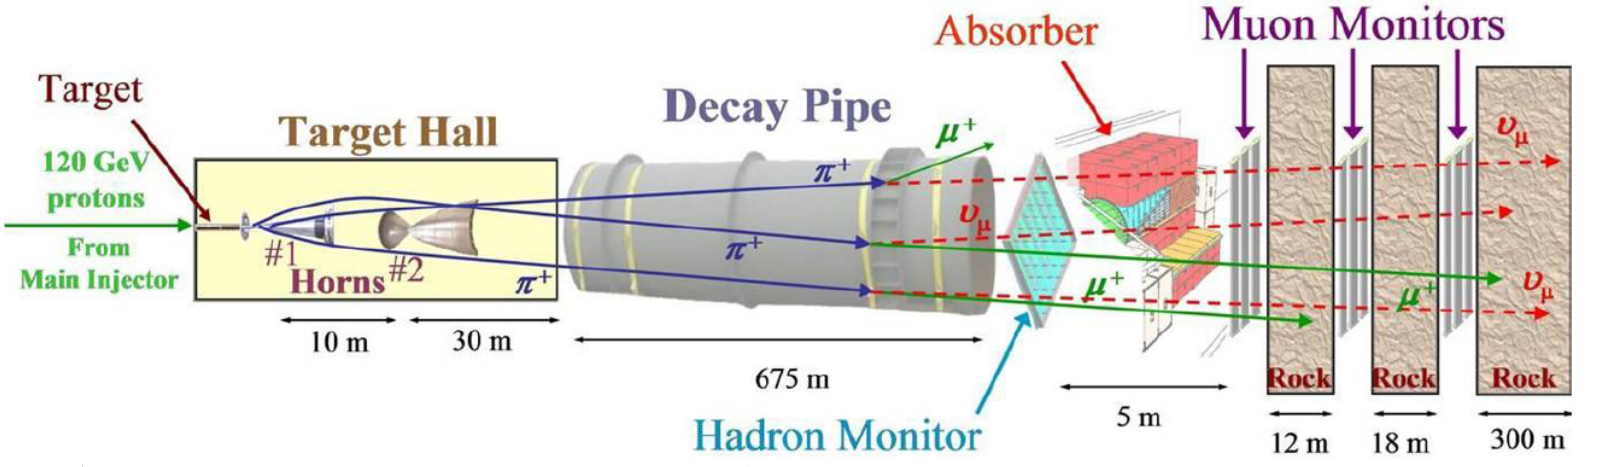
\includegraphics[width=\textwidth]{diagrams/4-chips/numi_beam.png}
    \caption[Schematic of the main components of the \numi beam.]
    {Schematic of the main components of the \numi beam (not to scale) shown with dimensions. The
        MINOS and \nova near detectors and the MINERvA experiment are located just to the right
        of what is shown. Figure taken from Ref.~\cite{adamson2016}.}
    \label{fig:numi_beam}
\end{figure}

Every \unit{1.33}{\mathrm{seconds}} a \unit{10}{\mu\mathrm{s}} long spill of protons accelerated
to \unit{120}{\GeV} by the Main Injector ring are directed towards a stationary graphite target.
The resulting interactions within the target create a shower of secondary hadrons containing
predominantly pions and kaons. The hadrons are passed through a focusing system of two magnetic
horns tuned principally to focus charged pions along the beamline while rejecting other particles.
After focusing, the surviving hadrons are allowed to decay in flight to a beam of muon neutrinos
in a \unit{675}{\mathrm{m}} long decay pipe via the processes,
\begin{align} % NUMI DECAY EQUATIONS %
    \pi^{+} & \rightarrow\mu^{+}+\nu_{\mu}, \label{eq:pi_decays}   \\
    K^{+}   & \rightarrow\mu^{+}+\nu_{\mu}. \label{eq:kaon_decays}
\end{align}
The resulting muons also decay such that $\mu^{+}\rightarrow e^{+}+\nu_{e}+\bar{\nu}_{\mu}$
producing an intrinsic $\nu_{e}$ background as well as wrong sign $\nu_{\mu}$ contamination.

Alternatively, the polarity of the horns can be used to switch the dominant sign of the hadrons
focused, allowing \numi to operate as either a neutrino or antineutrino beam. These two modes of
operation are called \emph{forward horn current} and \emph{reverse horn current} for primarily a
neutrino or antineutrino beam composition respectively. Any remaining hadrons, alongside
electrons, muons and surviving primary protons are absorbed by rock downstream of the decay pipe,
leaving just the neutrino components of the beam.

Long-baseline neutrino experiments typically consist of a \emph{near detector} to measure the beam
neutrino composition at source and a much larger \emph{far detector} to measure the oscillated
composition at many hundreds of kilometres. The \numi beamline contains three detectors just
downstream of \unit{300}{\mathrm{m}} of rock: The MINERvA spectrometer~\cite{mcfarland2006}, the
near detector for MINOS (now used by MINERvA), and the near detector for \nova. \chips prototypes
within the \numi beam will not have a dedicated near detector; therefore, data from the above
detectors will be crucial for physics analysis in order to constrain the beam composition and
flux.

The \numi neutrino beam passes through the Earth's crust until it finally emerges in northern
Minnesota. This is where the MINOS, \nova, and prototype \chips far detectors are located (used to
be located in the MINOS case), as shown in Fig.~\ref{fig:numi_map}. The Minnesota state nickname
`land of 10,000 lakes' is not an overstatement, with a vast number of potential lakes for \chips
detector deployment. Additionally, intense iron ore mining on the `Iron Range' provides many
suitable disused (and now flooded) mine pits. The exact \chipsfive prototype detector location is
discussed in greater detail in Section.~\ref{sec:chips_detector}.

\begin{figure} % CHIPS LOCATION IN NUMI DIAGRAM %
    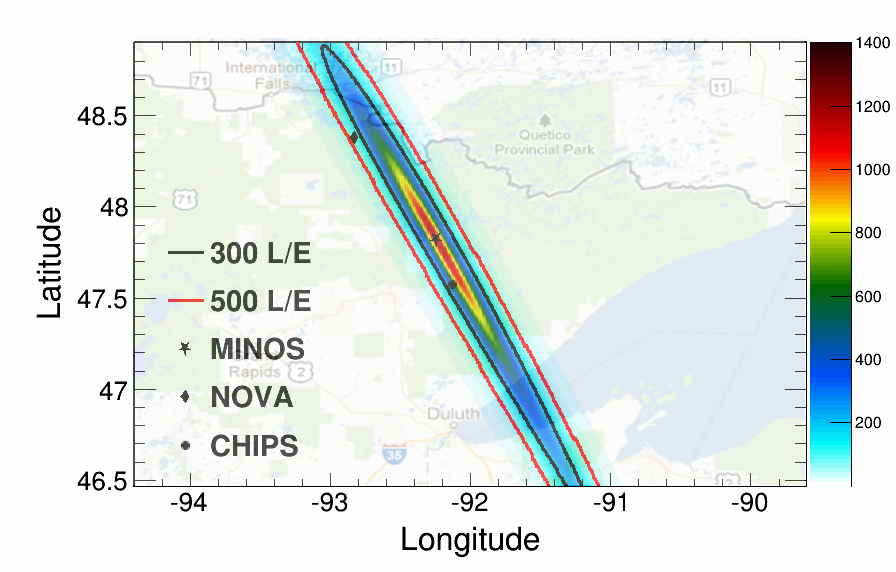
\includegraphics[width=0.7\textwidth]{diagrams/4-chips/numi_map.png}
    \caption[Map of detector locations in the \numi beam.]
    {Map of the MINOS, \nova and \chips locations in the \numi beam as it surfaces in northern
        Minnesota. Shown is the expected neutrino event rate assuming no oscillations, with lines
        of constant L/E indicated by contours. The western extent of Lake Superior can be seen in
        the lower right of the map. Image taken from Ref.\cite{adamson2013}.}
    \label{fig:numi_map}
\end{figure}

Due to the kinematics of pion decay, whether the far detector is placed directly on the beam axis
or not can have a significant impact on the observed energy spectrum of beam neutrinos as shown in
Fig.~\ref{fig:numi_axis}. For neutrinos directly on the beam axis, there is a strong energy
dependence on the parent pion energy from Eq.~\ref{eq:pi_decays}. However, as the off-axis angle
increases, the neutrino energy becomes less dependent on the parent pion energy and is restricted
to a narrowing range of decreasing energies. This effect known as the \emph{off-axis effect} is
used by both \nova and T2K to create a narrower energy spectrum focused on the
$\nu_{\mu}\rightarrow\nu_{e}$ oscillation maximum. Additionally, by reducing the tail of
higher-energy neutrinos, the number of background NC events can be greatly reduced, as is the case
for the \unit{7}{\mathrm{mrad}} off-axis \chipsfive prototype detector.

\begin{figure} % OFF-AXIS FLUX DIAGRAM %
    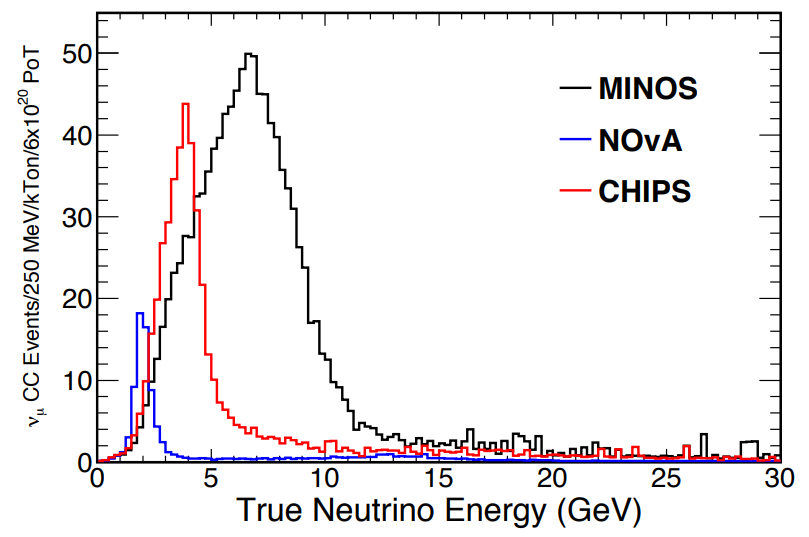
\includegraphics[width=0.6\textwidth]{diagrams/4-chips/numi_axis.png}
    \caption[Muon neutrino flux for different \numi detectors at different off-axis angles.]
    {Muon neutrino flux for different \numi detectors at different off-axis angles. Shown are the
        neutrino energy spectrum for MINOS (on-axis), \nova (\unit{14}{\mathrm{mrad}} off-axis),
        and \chipsfive (\unit{7}{\mathrm{mrad}} off-axis). Figure taken from
        Ref.~\cite{adamson2013}.}
    \label{fig:numi_axis}
\end{figure}

\subsection{Water Cherenkov detectors} %%%%%%%%%%%%%%%%%%%%%%%%%%%%%%%%%%%%%%%%%%%%%%%%%%%%%%%%%%%
\label{sec:chips_concept_cherenkov} %%%%%%%%%%%%%%%%%%%%%%%%%%%%%%%%%%%%%%%%%%%%%%%%%%%%%%%%%%%%%%

The \chips detector concept is based upon the water Cherenkov technique for neutrino detection. A
large body of target water is instrumented with photomultiplier tubes (PMTs) to record the
Cherenkov radiation produced by sufficiently relativistic charged particles resulting from
neutrino interactions. By using readily available water as the target material and only
instrumenting the volume surface, water Cherenkov detectors provide the best detection methodology
for maximising volume and reducing cost.

Cherenkov radiation is emitted by all electrically charged particles travelling faster than the
local phase velocity of light in a dielectric medium. Similar to the sonic boom created by a
supersonic aircraft, Cherenkov radiation forms a shock wave of coherent light, as shown in
Fig.~\ref{fig:cherenkov}. Typically the emitted light has wavelengths in the optical to
ultraviolet range. When projected onto the detector wall, the resulting cone of radiation
generates a distinctive ring shape. The cone opening angle (the angle at which light is emitted)
$\theta_{c}$ is given by:
\begin{equation}
    \cos\theta_{c} = \frac{1}{\beta n(\lambda)},
    \label{eq:cherenkov_angle}
\end{equation}
where $\beta=v/c$ and $n$ is the refractive index of the medium~\cite{particle2020}. Note that $n$
is a function of the wavelength of emission $\lambda$, and so is the opening angle. As the
refractive index of water is $\sim 1.33$ for typical wavelengths of emission, and using the
ultrarelativistic limit $\beta\sim 1$ the opening angle is found to be $\sim41^{\circ}$.

\begin{figure} % CHERENKOV EFFECT DIAGRAM DIAGRAM %
    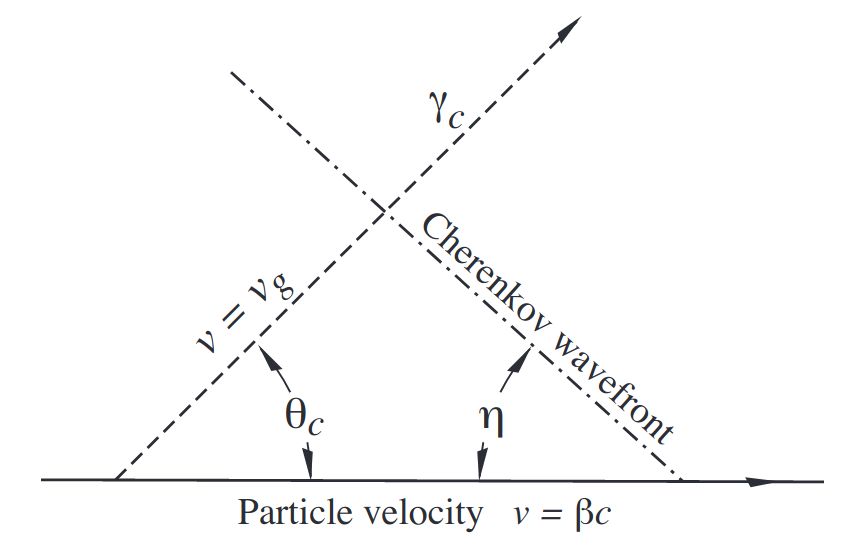
\includegraphics[width=0.6\textwidth]{diagrams/4-chips/cherenkov.png}
    \caption[Diagram of Cherenkov radiation emission.]
    {Diagram of Cherenkov radiation emission and wavefront angles. The angles $\theta_{c}$ and
        $\eta$ are not equal in a dispersive medium. Figure taken from Ref.~\cite{particle2020}}
    \label{fig:cherenkov}
\end{figure}

In Eq.~\ref{eq:cherenkov_angle} there is no Cherenkov emission when $\cos\theta_{c} > 1$, which is
the case when $\beta n(\lambda)<1$. Therefore, a Cherenkov energy threshold $E_{t}$ exists for
charged particle, which when expressed in terms of the particle mass $m$ is given by:
\begin{equation}
    E_{t} = \gamma m = \frac{m}{\sqrt{1-(1/n)^{2}}}.
    \label{eq:cherenkov_threshold}
\end{equation}
Again using $n\sim 1.33$, a threshold energy of $\sim1.5m$ is typical.

The number of Cherenkov photons emitted by a particle of charge $ze$ per unit wavelength per unit
path length is given by:
\begin{equation}
    \frac{d^{2}N}{d\lambda dx}=\frac{2\pi\alpha z^{2}}{\lambda^{2}}
    \left(1-\frac{1}{1-\beta^{2}n^{2}(\lambda)}\right),
    \label{eq:cherenkov_emission}
\end{equation}
where $\alpha$ is the fine structure constant~\cite{particle2020}. Integrating over the range of
wavelengths for which PMTs are typically sensitive, \unit{350}{\mathrm{nm}} to
\unit{650}{\mathrm{nm}}, and using $\beta\sim 1$ and $n\sim 1.33$ gives $\sim240$ photons emitted
per cm travelled by the charged particle~\cite{perch2017}.

By analysing the Cherenkov ring (or rings) of light recorded by the PMTs on the walls of the
detector, information about the charged particle (particles) within an event can be determined.
The underlying neutrino interaction can then be understood indirectly. Primarily the challenge for
accelerator beam water Cherenkov detectors is the identification and reconstruction of an electron
or muon ring likely to have been produced from a beam neutrino and not a cosmic ray. This event
topology indicates a beam CC $\nu_{e}$ or CC $\nu_{\mu}$ event respectively, rejecting NC and
cosmic events.

The basic shape of a Cherenkov ring can be used to tell which charged particle created it. Muons
are long-lived and typically travel many metres within the detector, producing a clean ring with
sharp edges. Conversely, electrons almost immediately initiate an electromagnetic shower;
therefore, the observed ring is the sum of all the rings produced from the individual electrons
and positrons within the shower. As a consequence, when compared to a muon ring, electron rings
are characteristically fuzzy. A factor of this difference can be seen in Fig.~\ref{fig:emission
    distance}, which shows how the total amount of Cherenkov radiation is emitted for both electrons
and muons as a function of distance from the interaction vertex.

\begin{figure} % EMISSION DISTANCE DIAGRAM %
    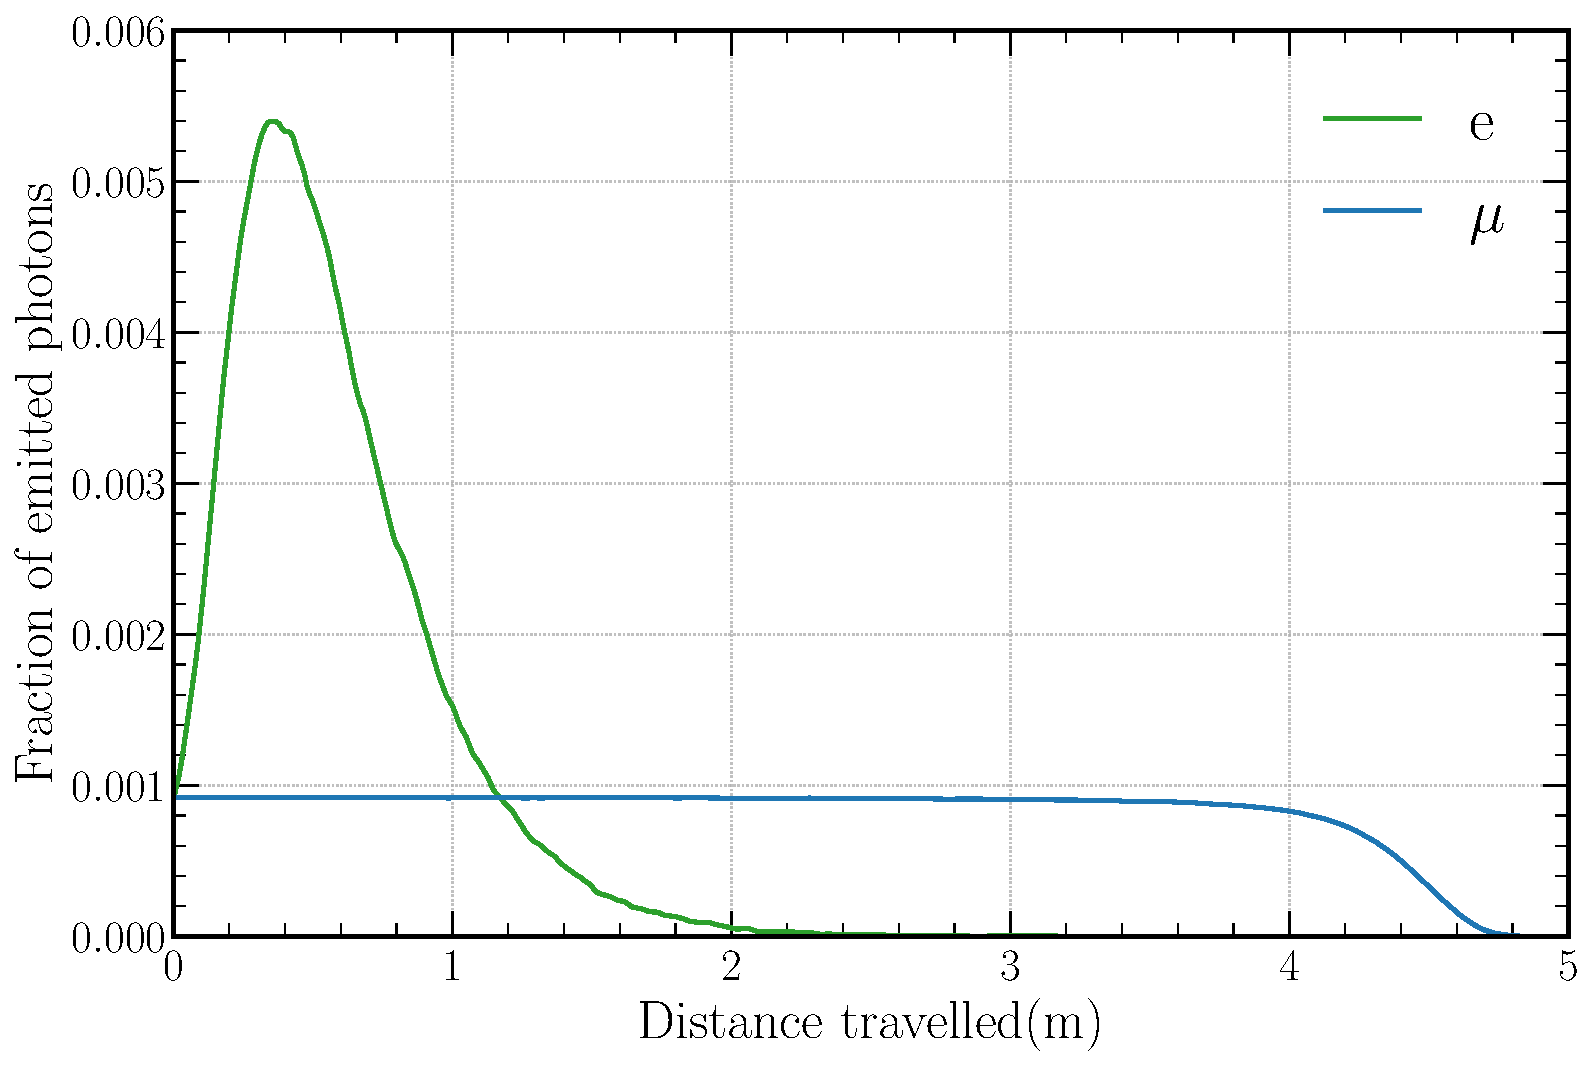
\includegraphics[width=0.6\textwidth]{diagrams/4-chips/emission_distance.pdf}
    \caption[Fraction of Cherenkov photons emitted as a function of distance.]
    {The fraction of the total number of photons emitted as a function of the distance from the
        interaction vertex for both electrons and muons with energy of \unit{2.5}{\GeV}. Multiple
        particles within the electron induced electromagnetic shower emit their Cherenkov
        radiation over a short distance and in slightly different directions. Conversely, a muon
        travels relatively much further emitting an approximately constant level of Cherenkov
        radiation as it does so, leading to a clean, sharp-edged ring.}
    \label{fig:emission distance}
\end{figure}

The situation becomes complicated when multiple charged particles above the Cherenkov threshold
are involved, common at multi-$\GeV$ energies. In this case, multiple overlapping rings are
observed, making reconstruction difficult. The worst-case scenario, however, is when two rings
entirely overlap, removing any ability to tell them apart. This topology is commonly the case for
NC interactions producing a $\pi^{0}$ in the final state, forming the primary background for CC
$\nu_{e}$ appearance.

$\pi^{0}$ particles decay to a pair of photons with a 98.82\% branching ratio, both which almost
immediately initiate an electromagnetic shower, just like an electron~\cite{particle2020}. This
process leads to two, electron like rings to be observed with a separation angle given by:
\begin{equation}
    (1-\cos\theta_{ij})=\frac{m_{\pi}^2}{2E_{i}E_{k}},
\end{equation}
where $m_{\pi}$ is the invariant mass of the $\pi^{0}$ and $E_{i}$ and $E_{j}$ are the energies of
the two photons respectively. Therefore, for a $\pi^{0}$ decaying to two \unit{1}{\GeV} photons,
there is just $\sim 8^{\circ}$ of separation between the rings, making them difficult to tell
apart. This distinction is especially hard when electron like rings are also fuzzy. Alternatively,
if the two photons have an unequal energy distribution, such that one is much more energetic than
the other, the higher energy photon ring can dominate, and the other can not be identified,
leading to what looks like a single electron ring, again a misidentification.

\section{The \chipsfive detector} %%%%%%%%%%%%%%%%%%%%%%%%%%%%%%%%%%%%%%%%%%%%%%%%%%%%%%%%%%%%%%%%
\label{sec:chips_detector} %%%%%%%%%%%%%%%%%%%%%%%%%%%%%%%%%%%%%%%%%%%%%%%%%%%%%%%%%%%%%%%%%%%%%%%

\chipsfive is the first large scale prototype detector module for the \chips project. A
\unit{25}{\mathrm{m}} wide and \unit{12}{\mathrm{m}} high cylinder once fully deployed, \chipsfive
has an inner surface area of \unit{1924}{\mathrm{m}^2} and a total target mass
\unit{5.9}{\mathrm{kton}}. Via the process of design, construction, deployment, and data taking,
\chipsfive primarily aims to refine the \chips concept for future full-scale
($\sim$\unit{15}{\mathrm{kton}}) modules. Consequently, \chipsfive is designed such that the
details outlined in this section are fully characteristic of what a full-sized \chips module is
envisioned to be. Here, the location, structure, instrumentation, water filtration, deployment,
and current status are presented. The full electronics and DAQ details are outlined in
Chapter.~\ref{chap:daq}.

\subsection{Location} %%%%%%%%%%%%%%%%%%%%%%%%%%%%%%%%%%%%%%%%%%%%%%%%%%%%%%%%%%%%%%%%%%%%%%%%%%%
\label{sec:chips_detector_location} %%%%%%%%%%%%%%%%%%%%%%%%%%%%%%%%%%%%%%%%%%%%%%%%%%%%%%%%%%%%%

\chipsfive is located at the Wentworth 2W pit in northern Minnesota, USA, near the small town of
Hoyt Lakes. A disused and flooded surface Taconite ore (a type of iron ore) mine pit, Wentworth 2W
is located \unit{7}{\mathrm{mrad}} off the \numi axis at a distance of \unit{712}{\mathrm{km}}
from the beam target. Roughly \unit{0.8}{\mathrm{km}}$\times$\unit{1.2}{\mathrm{km}} in size with
a maximum depth of \unit{60}{\mathrm{m}} ($\pm$\unit{3}{\mathrm{m}} throughout the year), the pit
allows for an overburden of approximately \unit{50}{\mathrm{m}} with \chipsfive resting at the
bottom. With an average daily low temperate of $-24^{\circ}\mathrm{C}$ in January, the pit freezes
over during the winter months, therefore, work is only possible during the summer months of May to
October.

A sizeable earthen ramp on the south side of the Wentworth 2W pit is used for construction on
land. The construction site is easily accessible by road and well connected to power, due to the
heavy infrastructure in place for mining. Additionally, the nearby PolyMet mining administration
building is used as a laboratory environment for construction and testing of individual components
before installation within the detector. A labelled satellite view of Wentworth 2W is given in
Fig.~\ref{fig:pit} for context, with a picture of the construction site shown in
Fig.~\ref{fig:from_the_sky}.

\begin{figure} % PIT DIAGRAM %
    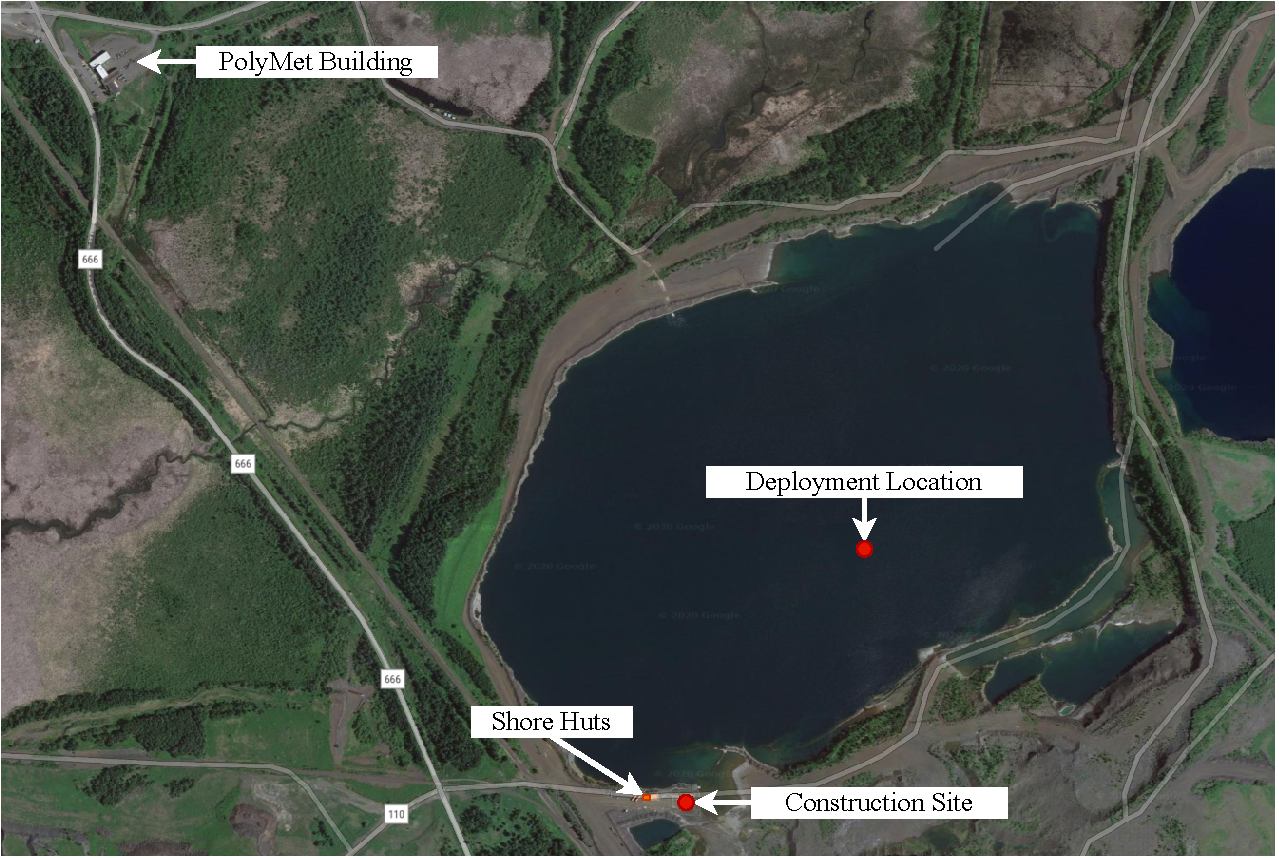
\includegraphics[width=\textwidth]{diagrams/4-chips/pit.pdf}
    \caption[Satellite view of the Wentworth 2W mine pit, with key locations.]
    {Satellite view of the Wentworth 2W flooded mine pit in northern Minnesota, showing key
        \chipsfive locations. The PolyMet building, shore huts, construction site and deployment
        location are shown. For both the construction site and deployment location the red circle
        shows the \chipsfive detector size to scale.}
    \label{fig:pit}
\end{figure}

\begin{figure} % CHIPS FROM THE SKY DIAGRAM %
    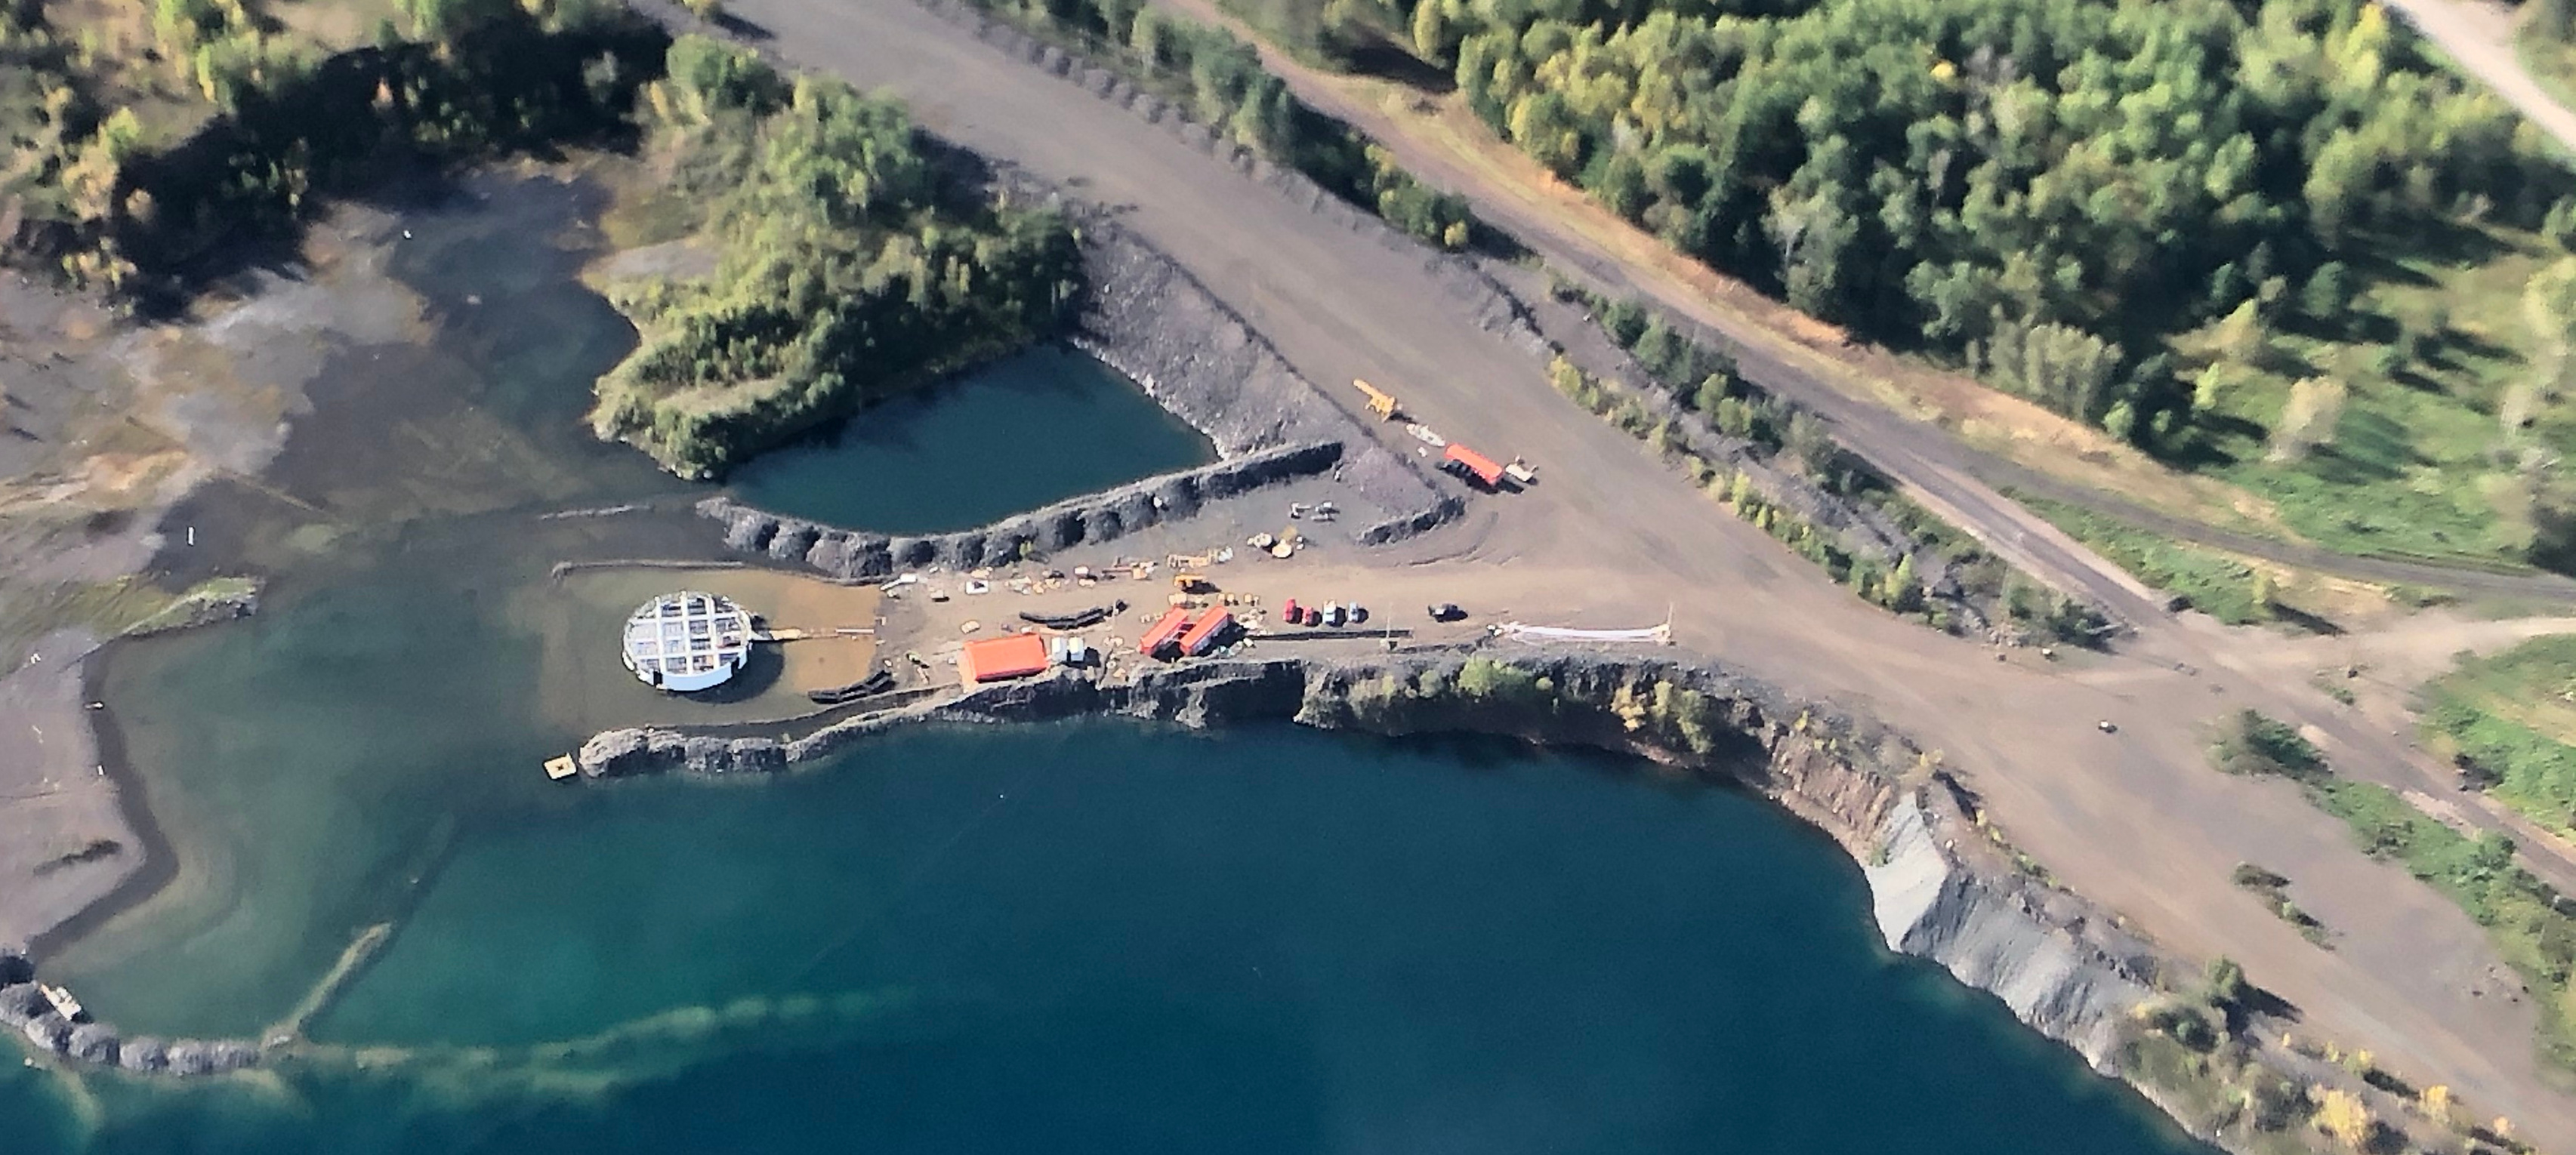
\includegraphics[width=\textwidth]{diagrams/4-chips/from_the_air.jpeg}
    \caption[Picture of the \chipsfive construction site from the air.]
    {Picture of the \chipsfive construction site from the air facing south. The Wentworth 2W pit
        is in the lower half of the image, with the part built \chipsfive detector visible at the
        bottom of the earthen construction ramp. The two white shore huts can just be seen halfway
        up the ramp.}
    \label{fig:from_the_sky}
\end{figure}

\subsection{Structure} %%%%%%%%%%%%%%%%%%%%%%%%%%%%%%%%%%%%%%%%%%%%%%%%%%%%%%%%%%%%%%%%%%%%%%%%%%%
\label{sec:chips_detector_structure} %%%%%%%%%%%%%%%%%%%%%%%%%%%%%%%%%%%%%%%%%%%%%%%%%%%%%%%%%%%%%

The structure of the \chipsfive detector module consists primarily of two \unit{26}{\mathrm{m}}
diameter and \unit{1.3}{\mathrm{m}} high lightweight stainless steel circular \emph{endcaps} that
form the top and bottom of the cylinder. During construction on land the conveniently named
\emph{top-cap} is held above the \emph{bottom-cap} by \unit{1.5}{\mathrm{m}} long steel struts as
shown in Fig.~\ref{fig:frame}. This configuration allows for the endcap instrumentation, detailed
in Section.~\ref{sec:chips_detector_instrumentation}, to be easily installed.

\begin{figure} % CHIPS FRAME DIAGRAM %
    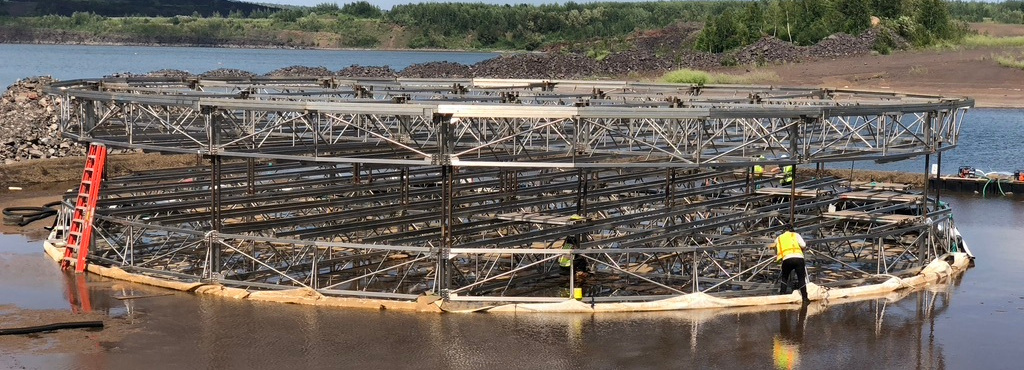
\includegraphics[width=\textwidth]{diagrams/4-chips/frame.jpeg}
    \caption[Picture of the \chipsfive structural frame.]
    {Picture of the \chipsfive structural frame, with humans for scale. The top and bottom endcaps
        can be seen separated by steel struts. Rows of stainless steel \emph{stringers}
        are attached to the inside of each endcap to mount the instrumentation.}
    \label{fig:frame}
\end{figure}

The two endcaps are connected by 28 \unit{12}{\mathrm{m}} long Dyneema cables around their
perimeter. Additionally, 48 \unit{16}{\mathrm{inch}} diameter air-filled PVC pipes are attached to
the frame of the top-cap, making it buoyant. Therefore, once deployed into the pit, the bottom-cap
sinks while the top-cap floats, this pulls the Dyneema cable until taut, forming the final
expanded detector shape, as shown in Fig.~\ref{fig:chips_render}.

\begin{figure} % CHIPS RENDER DIAGRAM %
    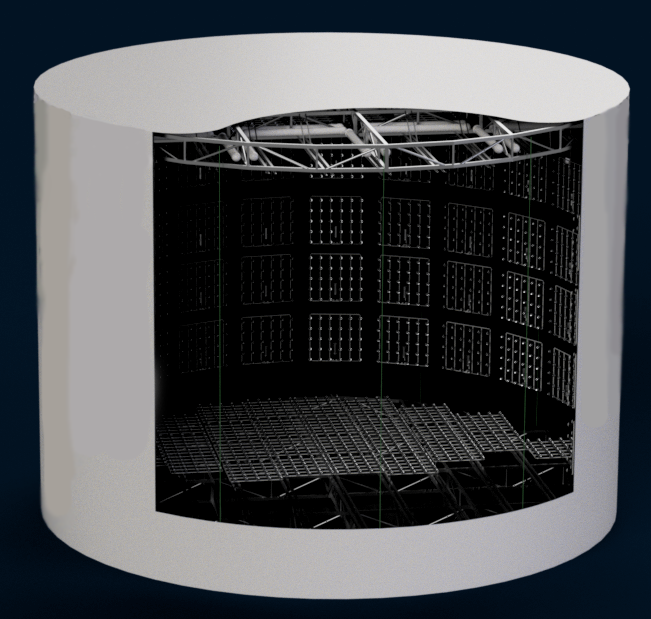
\includegraphics[width=0.6\textwidth]{diagrams/4-chips/chips_render_1.png}
    \caption[Graphical rendering of the \chipsfive detector.]
    {Graphical rendering of the fully deployed and expanded \chipsfive detector module with a
        section of the liner cutaway. The bottom endcap and wall planes are visible, as well as
        the top endcap structure and floatation. The green lines indicate the Dyneema cables
        holding the top-cap and bottom-cap together.}
    \label{fig:chips_render}
\end{figure}

A lightproof and watertight liner is also installed to surround the fully expanded structure.
Designed to isolate the clean internal water from the external pit water and to prevent
non-Cherenkov light from reaching the PMTs, the liner is made from geomembrane, a flexible
reinforced polymer membrane. Commercially available in large rolls the liner is welded together
during construction to form the top, bottom, and sides. Note that when fully deployed, the liner
does not take any of the structural strain.

\subsection{Instrumentation} %%%%%%%%%%%%%%%%%%%%%%%%%%%%%%%%%%%%%%%%%%%%%%%%%%%%%%%%%%%%%%%%%%%%%
\label{sec:chips_detector_instrumentation} %%%%%%%%%%%%%%%%%%%%%%%%%%%%%%%%%%%%%%%%%%%%%%%%%%%%%%%

The \chipsfive detector is instrumented with PMTs arranged within distinct plane like structures
called Planar Optical Modules (POMs), which take inspiration from the Digital Optical Modules
(DOMs) used by IceCube and KM3NeT~\cite{hanson2006, eijk2015}. Each POM is a roughly
\unit{2}{\mathrm{m}}$\times$\unit{3}{\mathrm{m}} array of watertight PVC tubing equipped with
anywhere between $15$ to $30$ PMTs, in addition to the lowest level of DAQ electronics and power
distribution. Standard commercially available schedule $40$ PVC piping and connectors are used to
form the structure of each plane, bound together with PVC primer and cement.

There are two types of POM used within \chipsfive, differentiated by the PMTs and the data
acquisition electronics they use and named after the institution at which they were developed.
Firstly, \emph{Nikhef} POMs use \unit{88}{\mathrm{mm}} HZC PMTs with electronics developed by the
KM3NeT experiment~\cite{katz2009, adrian2016}. Secondly, \emph{Madison} POMs use
\unit{3}{\mathrm{inch}} Hamamatsu R6091 PMTs donated from the NEMO3 experiment~\cite{arnold2005}
with novel electronics developed by \chips in collaboration with the Wisconsin IceCube Particle
Astrophysics Centre (WIPAC) in Madison, Wisconsin. The \unit{88}{\mathrm{mm}} HZC PMTs have a high
ratio of output electrons to incident photons (quantum efficiency) of 24.4\% at a wavelength of
\unit{400}{\mathrm{nm}}, compared to the low 12.0\% ratio achieved by the R6091 PMTs. Furthermore,
the first photon time resolution is $\sim2\mathrm{ns}$ and $\sim$\unit{5}{\mathrm{ns}} for
\unit{88}{\mathrm{mm}} HZC and R6091 PMTs respectively.

In total $6114$ \unit{88}{\mathrm{mm}} HZC and $450$ Hamamatsu R6091 PMTs are arranged into $226$
Nikhef and $30$ Madison POMs. Every PMT is housed in an assembly as shown in
Fig.~\ref{fig:nikhef_pmt_assembly} for the Nikhef case and Fig.~\ref{fig:madison_pmt_assembly} for
the Madison case. Importantly, to increase the level of light collection, each Nikhef PMT is
equipped with a \emph{light-cone} consisting of a circular reflective surface at \unit{45}{^\circ}
to the PMT normal. The Madison PMT assembly is similar but has no cover or light cone. For POMs
attached to either endcap, their PMTs are angled at \unit{45}{^\circ} facing the direction of the
beam to increase light collection furthermore.

All PMTs within a POM are connected to the lowest level of DAQ electronics contained within a
dedicated electronics box. Either an aluminium or PVC cylinder in the Nikhef or Madison case
respectively. A flexible PVC \emph{pigtail} is attached to each POM electronics box containing
connections to the higher level DAQ and power supply. A \emph{water-block} within each pigtail
ensures that even if the outside connection is flooded, every POM is capable of withstanding the
\unit{6}{\mathrm{atm}} of water pressure at the bottom of the pit. A fully assembled and installed
Nikhef POM is shown in Fig.~\ref{fig:single_plane} for reference.

\begin{figure} % NIKHEF PMT ASSEMBLY DIAGRAM %
    \centering
    \subcaptionbox{Disassembled}{%
        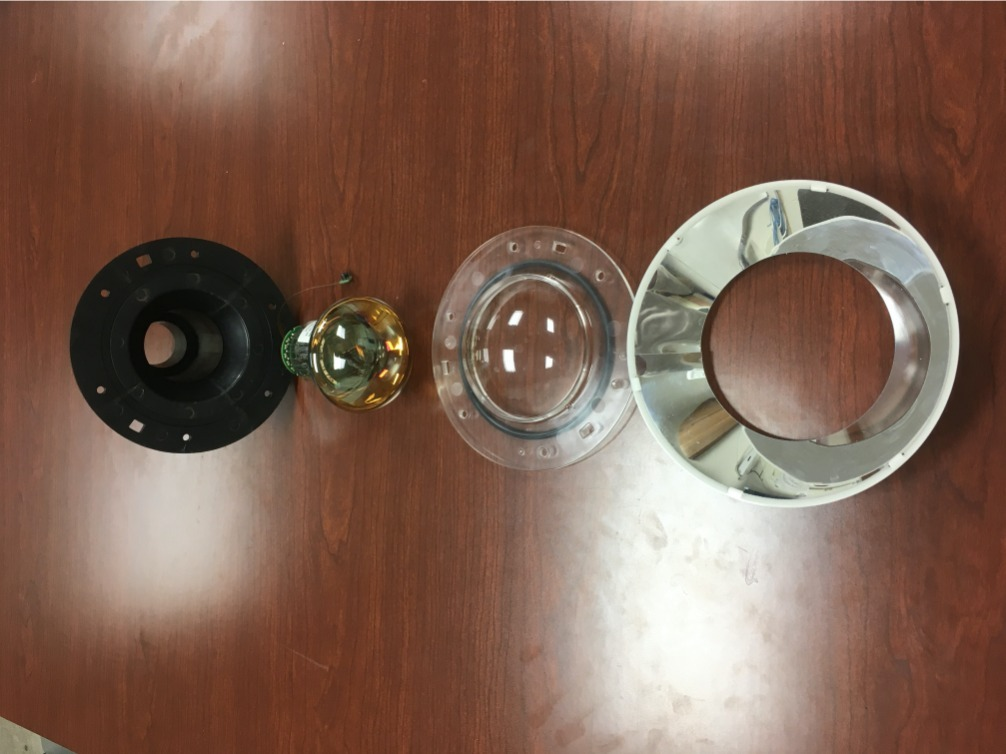
\includegraphics[height=5.5cm]{diagrams/4-chips/pmt_disassembled.jpg}%
    }
    \quad
    \subcaptionbox{Assembled}{%
        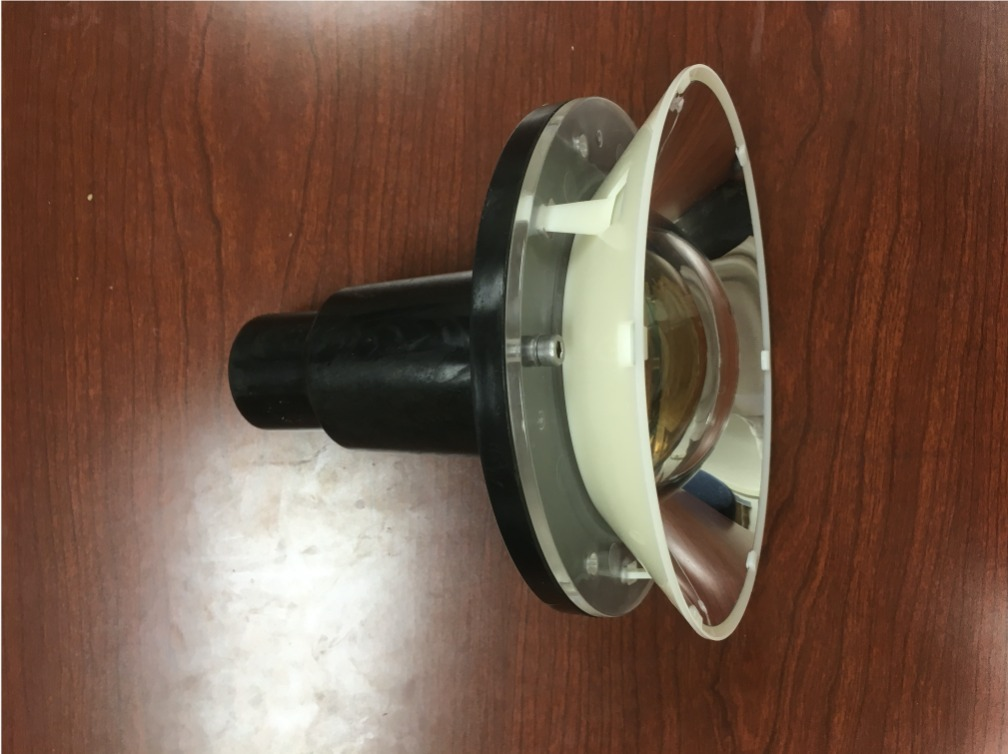
\includegraphics[height=5.5cm]{diagrams/4-chips/pmt_assembled.jpg}%
    }
    \caption[Disassembled and assembled Nikhef PMT housing components.]
    {Disassembled (a) and assembled (b) Nikhef PMT assembly components. The assembly comprises of
        a black PVC insert, a \unit{88}{\mathrm{mm}} HZC PMT, a transparent acrylic cover, and a
        reflective light cone. The PMT is glued to the inside surface of the cover using a
        silicone-based optical gel and a watertight seal is made between the insert and cover
        using an O-ring. The reflective light cone is clipped to the front of the cover and the
        whole assembly is glued into the POM PVC structure.}
    \label{fig:nikhef_pmt_assembly}
\end{figure}

\begin{figure} % MADISON PMT ASSEMBLY DIAGRAM %
    \centering
    \subcaptionbox{Outside}{%
        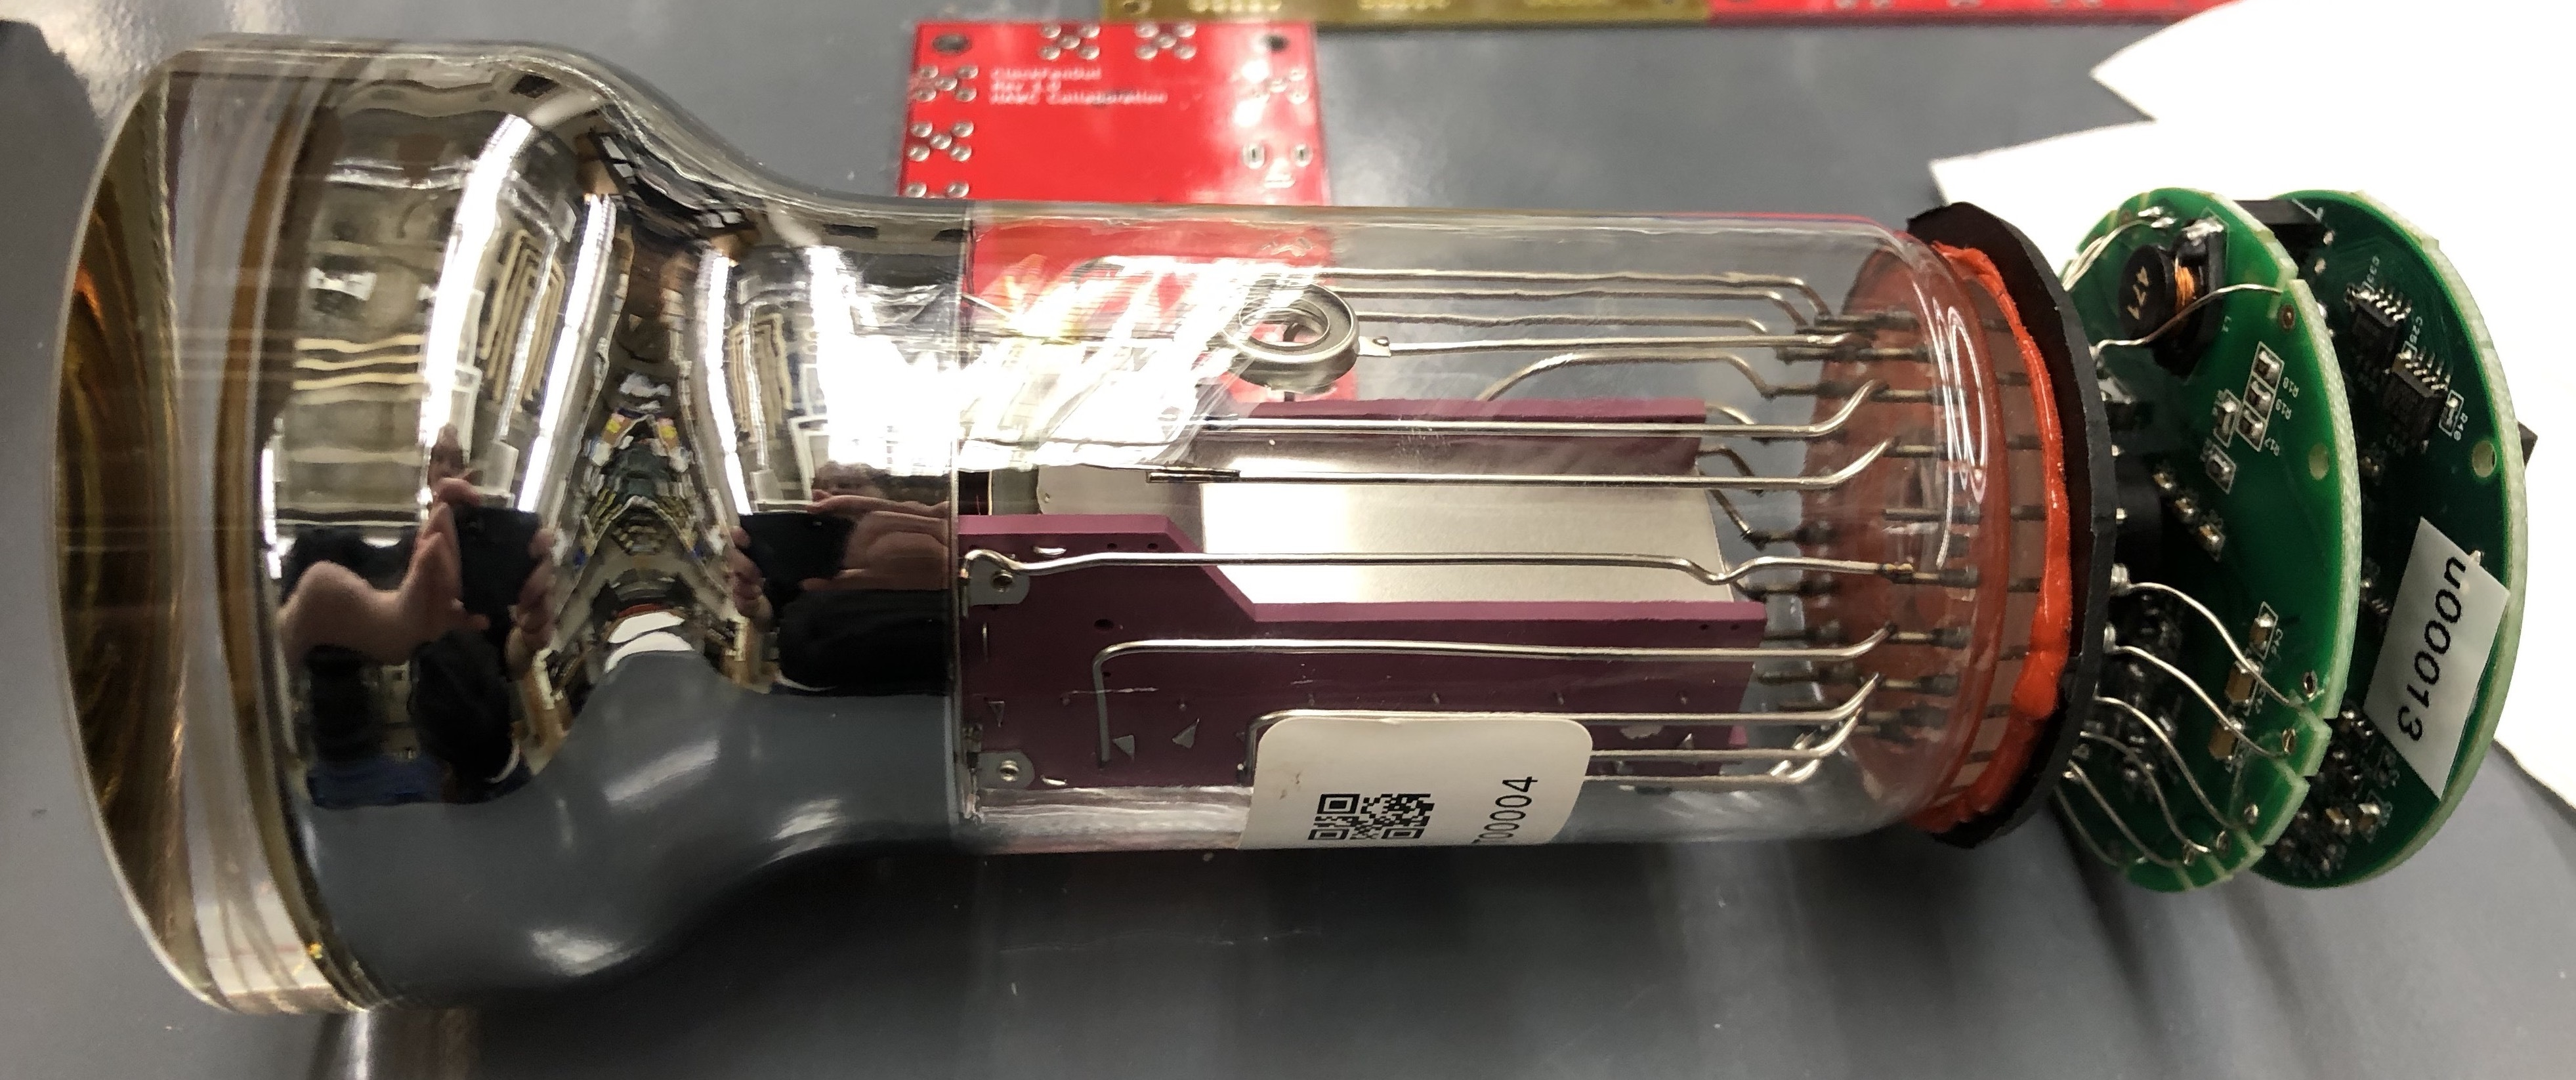
\includegraphics[angle=270,origin=c,height=4.3cm]{diagrams/4-chips/madison_pmt.jpeg}%
    }
    \quad
    \subcaptionbox{Inside}{%
        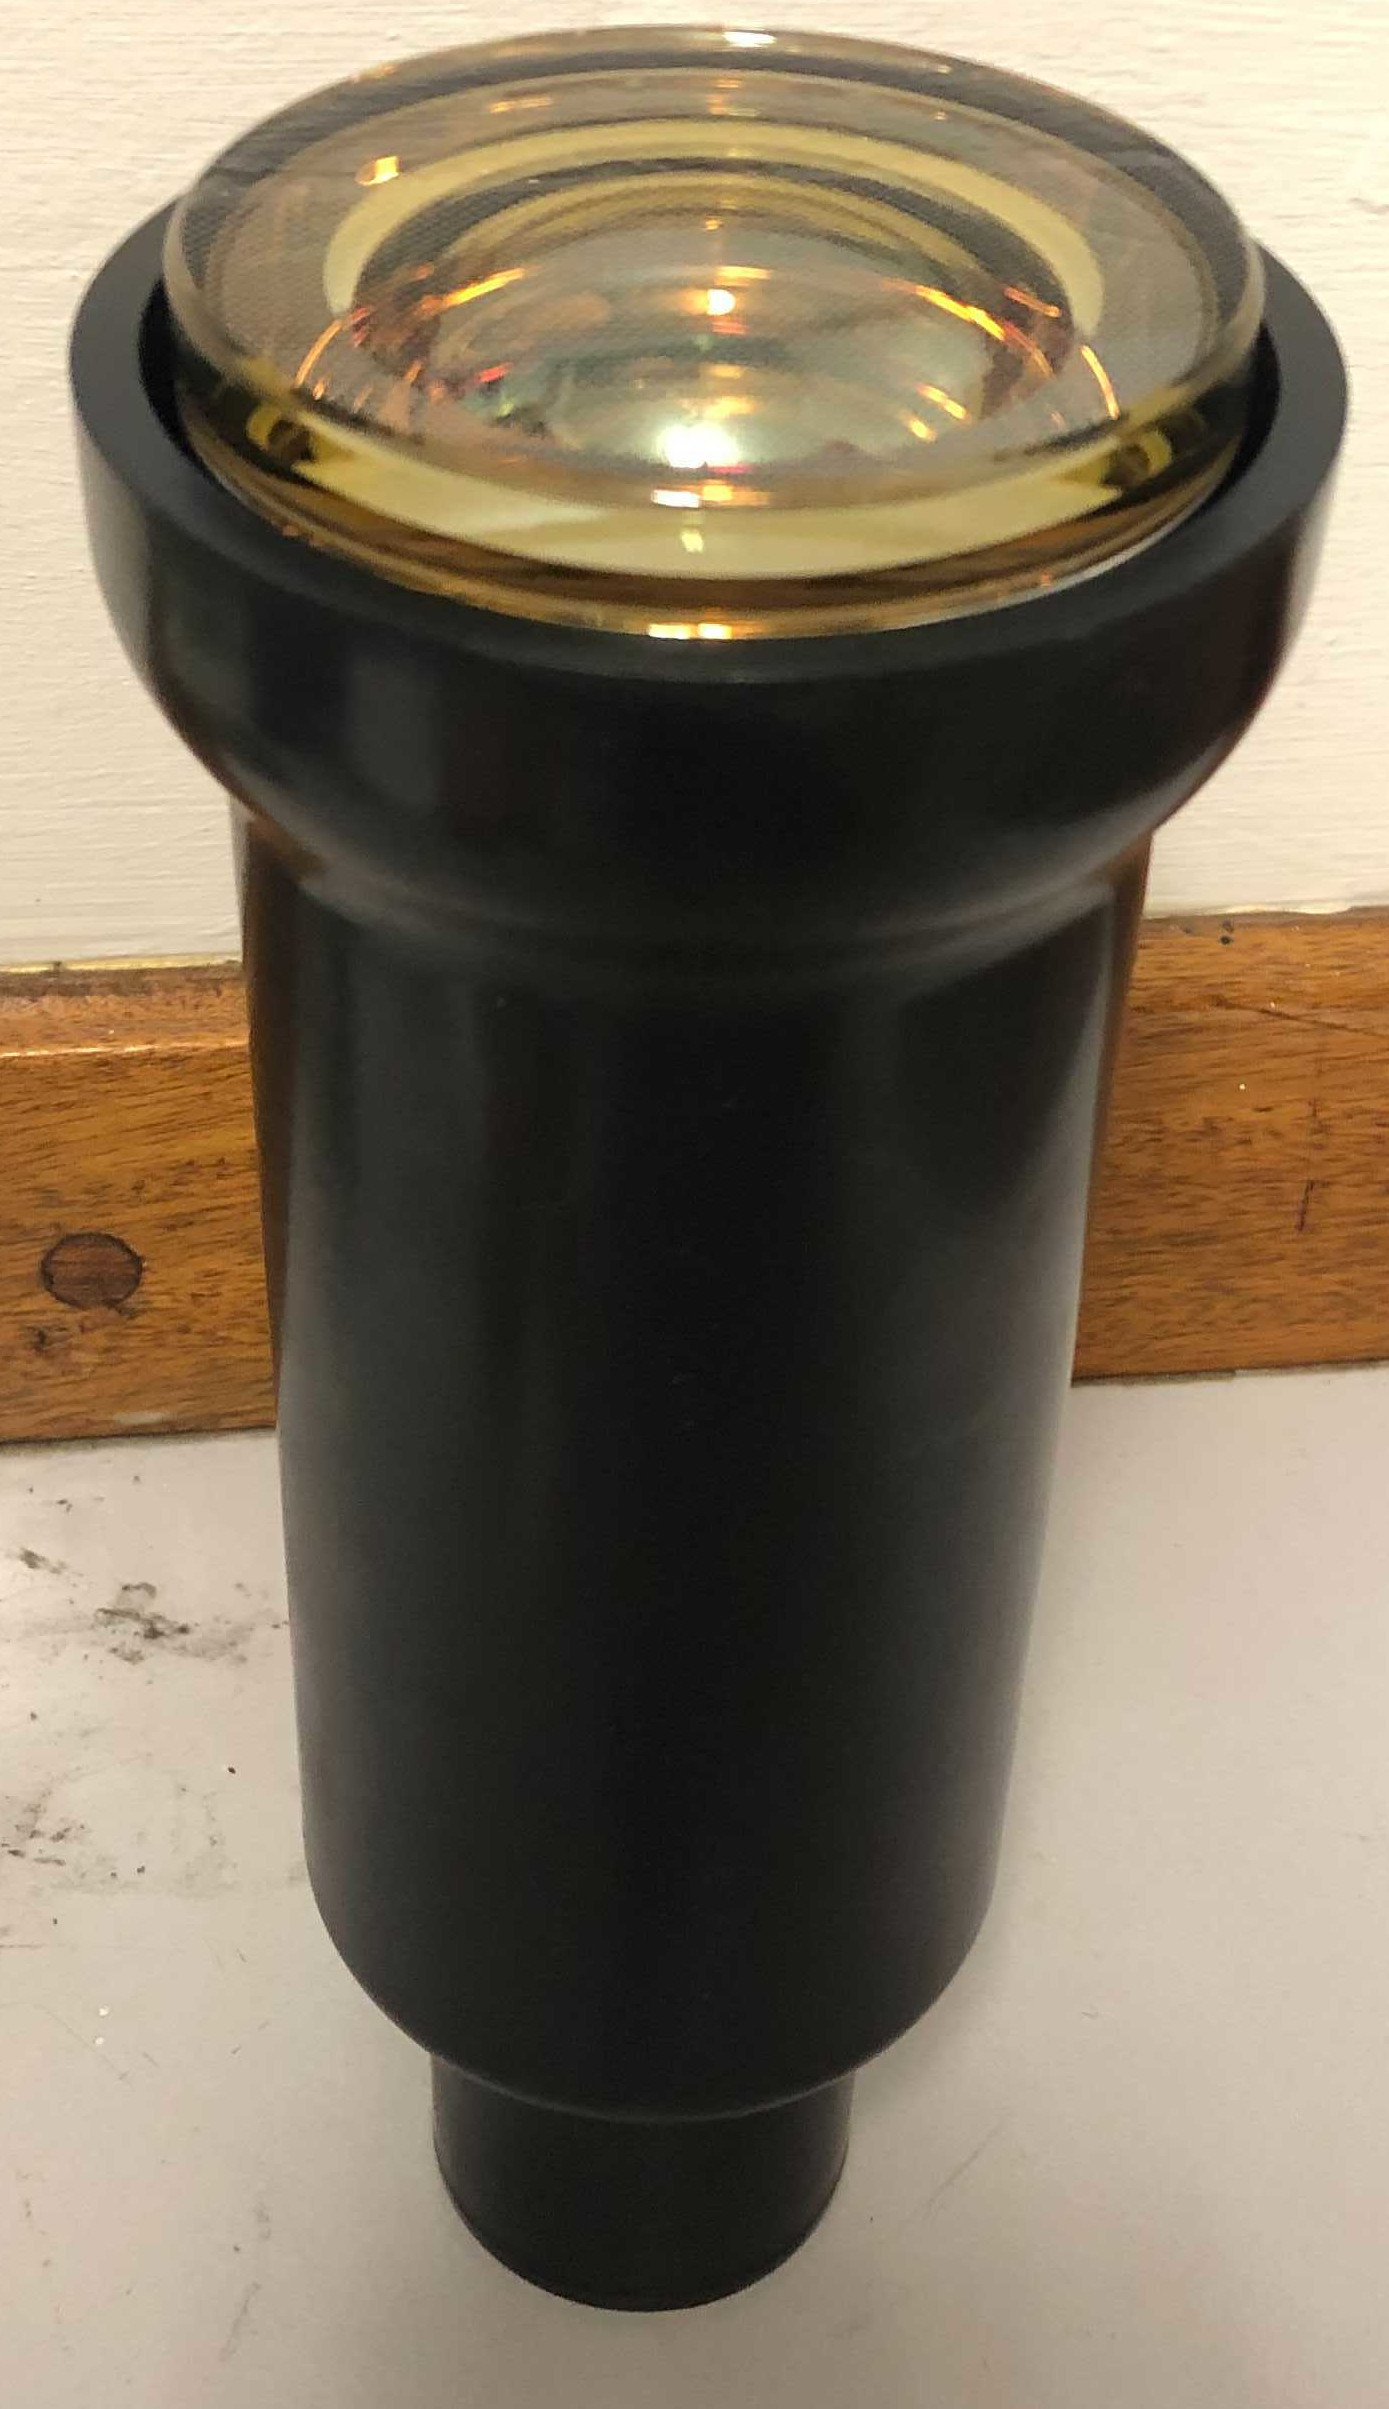
\includegraphics[height=6cm]{diagrams/4-chips/madison_assembly.jpg}%
    }
    \caption[Madison POM PMT assembly.]
    {A Hamamatsu R6091 Madison POM PMT outside (a) and inside its insert (b). The PMT is
        \emph{potted} inside its black PVC insert creating a watertight seal that can withstand
        the \unit{6}{\mathrm{atm}} of water pressure at the bottom of the pit.}
    \label{fig:madison_pmt_assembly}
\end{figure}

\begin{figure} % NIKHEF POM DIAGRAM %
    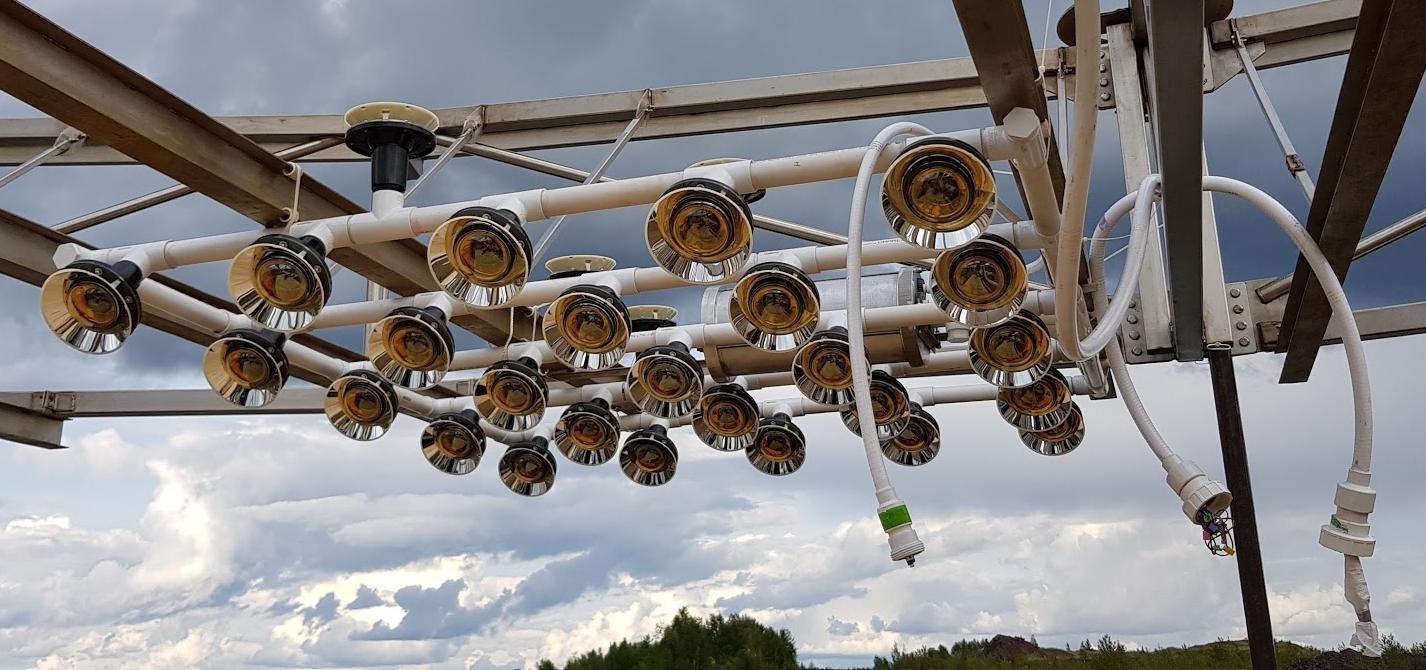
\includegraphics[width=\textwidth]{diagrams/4-chips/single_plane.jpg}
    \caption[Picture of a Nikhef POM.]
    {Picture of a single Nikhef full density POM installed on the top-cap of the \chipsfive
        detector. Both the inward-facing and veto PMTs are visible as well as the aluminium
        electronics container and pigtail whose end is covered in green tape.}
    \label{fig:single_plane}
\end{figure}

The POMs are tiled next to each other on the detector walls, attached to either the stainless
steel \emph{stringers} on the top-cap and bottom-cap, or clipped to the Dyneema cables on the
vertical walls of the \emph{barrel}. As mentioned previously, full high density and high coverage
detector instrumentation is not required for \chips detector modules, due to two main reasons.
Firstly, only highly directional accelerator beam events are to be studied. Therefore, the vast
majority of neutrino interaction Cherenkov radiation is deposited on a relatively small downstream
region of the detector walls. Secondly, beam neutrinos predominantly have multi-$\GeV$ energies,
yielding a relatively large amount of Cherenkov radiation. Therefore, a lower number of PMTs is
required to capture adequate Cherenkov radiation from an interaction.

Consequently, the distribution of the percentage of the detector walls covered by sensitive PMT
surface area (\emph{photocathode coverage}) is optimised to reduce the total number of PMTs. The
detector is split into three distinct regions of PMT photocathode coverage whose boundaries are
roughly defined by their azimuth angle $\phi$ from the centre of the downstream wall (at
$\phi=0^{\circ}$). Firstly, a \emph{full-density} Nikhef POM region in the most downstream
$\phi=\pm75^{\circ}$ region of the detector with a $\sim3\%$ photocathode coverage. Secondly, a
\emph{half-density} Nihkef POM region covering the $\phi=\pm75^{\circ}$ to $\phi=\pm180^{\circ}$
region of the endcaps and the $\phi=\pm75^{\circ}$ to $\phi=\pm140^{\circ}$ region of the barrel
with a $\sim1.5\%$ photocathode coverage. Finally, a \emph{half-density} Madison POM region
covering the $\phi=\pm140^{\circ}$ to $\phi=\pm180^{\circ}$ upstream region of the barrel with a
$\sim0.8\%$ photocathode coverage. Studies have shown that this configuration does not reduce
performance while vastly reducing the number of required PMTs~\cite{blake2016}.

Compared to the $\sim40\%$ uniform photocathode coverage of Super-Kamiokande, the \chipsfive
instrumentation configuration highlights just how significantly different detector design can be
when only studying accelerator beam neutrinos. Of importance to note is that photocathode coverage
in the upstream regions of the detector is still required, even if very low, for cosmic muon and
NC event rejection.

To further help with cosmic muon rejection, the \chipsfive detector module is equipped with a veto
region within the top-cap frame structure. Separated from the main detector volume by a
geomembrane liner, the \unit{1.3}{\mathrm{m}} high region can reject predominantly downward cosmic
muons by detecting the Cherenkov radiation they produce. $324$ \unit{88}{\mathrm{mm}} HZC PMTs are
included within the Nikhef POMs attached to the top-cap facing upwards leading to a veto
photocathode coverage of $\sim0.6\%$. A graphical rendering of all the top-cap POMs is shown in
Fig.~\ref{fig:top_cap}.

\begin{figure} % TOP CAP RENDER DIAGRAM %
    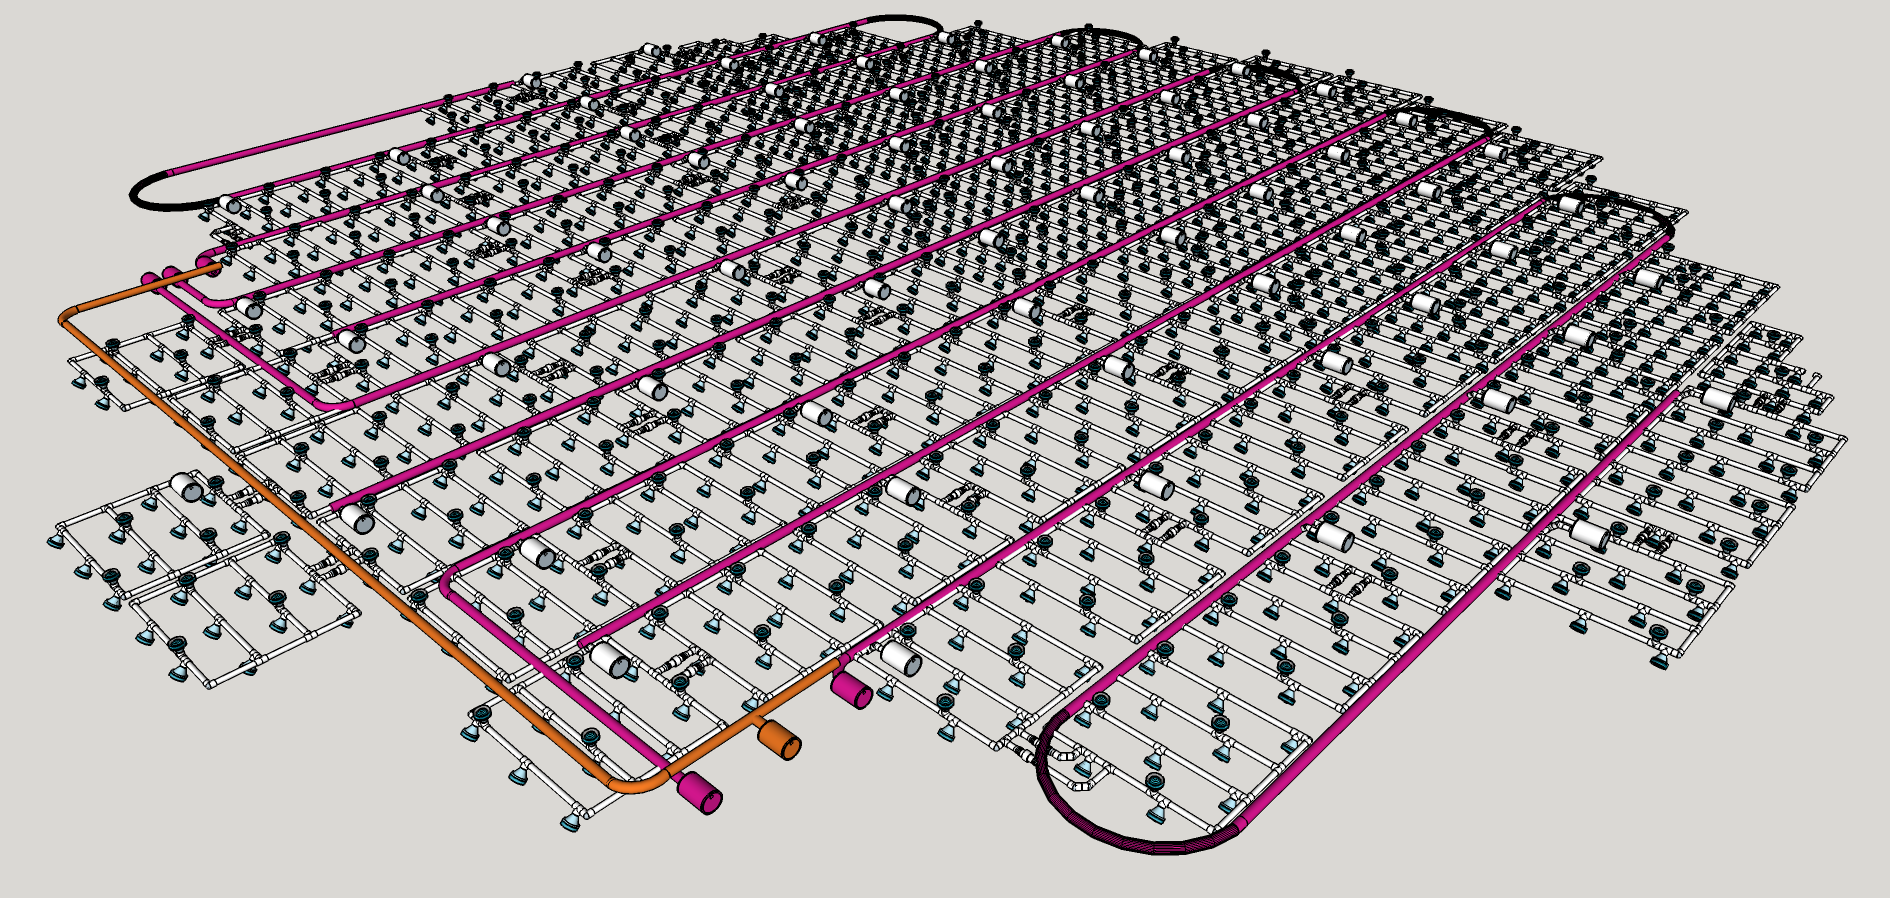
\includegraphics[width=\textwidth]{diagrams/4-chips/top_cap.png}
    \caption[Graphical rendering of the top-cap POMs.]
    {Graphical rendering of the top-cap POMs. Both the different photocathode coverage regions and
        the veto PMTs are visible.}
    \label{fig:top_cap}
\end{figure}

The detector instrumentation receives power and is connected to the highest level DAQ systems
through a \unit{500}{\mathrm{m}} long flexible PVC umbilical resting on the pit floor. The
umbilical contains two optical fibres for data and two shielded gauge 14 cables for power. One end
of the umbilical is attached to the bottom-cap of the detector while the other enters a hut on
shore containing the power supply and highest level DAQ equipment.

\subsection{Filtration} %%%%%%%%%%%%%%%%%%%%%%%%%%%%%%%%%%%%%%%%%%%%%%%%%%%%%%%%%%%%%%%%%%%%%%%%%%
\label{sec:chips_detector_water} %%%%%%%%%%%%%%%%%%%%%%%%%%%%%%%%%%%%%%%%%%%%%%%%%%%%%%%%%%%%%%%%%

Through surprisingly clear, in order to reach the desired $\sim$\unit{30}{\mathrm{m}} attenuation
length of light, the Wentworth 2W pit water still requires filtration to remove particulates and
bacteria. Therefore 2 (one to, one from) flexible umbilical tubes run from the detector to a hut
on shore containing filtration equipment. A pump passes the full detector water volume through a
series of $n$ carbon? commercially available filters every \unit{10}{days}. Studies have
shown~\cite{campbell2020} that this simple procedure allows for the desired attenuation length to
be reached after $n$ months of initial filtration. Additionally, the water within \chipsfive is
kept at a small positive pressure relative to the external pit water to prevent the entry of
particulates and bacteria though any small gaps in the liner.

\subsection{Construction and deployment} %%%%%%%%%%%%%%%%%%%%%%%%%%%%%%%%%%%%%%%%%%%%%%%%%%%%%%%%%
\label{sec:chips_detector_deployment} %%%%%%%%%%%%%%%%%%%%%%%%%%%%%%%%%%%%%%%%%%%%%%%%%%%%%%%%%%%%

- How it can grow if needed - buoyant top cap anchored to the bottom one, which when fully
deployed will rest on the bottom of the pit.

\subsection{Current status} %%%%%%%%%%%%%%%%%%%%%%%%%%%%%%%%%%%%%%%%%%%%%%%%%%%%%%%%%%%%%%%%%%%%%%
\label{sec:chips_detector_status} %%%%%%%%%%%%%%%%%%%%%%%%%%%%%%%%%%%%%%%%%%%%%%%%%%%%%%%%%%%%%%%%

During the summers of 2018 and 2019 extensive construction work for the \chipsfive detector was
carried out by a team of approximately 15 collaborators at any one time. By late summer 2019 is
became apparent that deployment of a fully instrumented \chipsfive detector before the freezing of
the lake in October would not be possible. Therefore, the decision was taken to only partly
instrument the top-cap and bottom-cap

- No liner between veto and main volume!
- In the summer of 2018 and 2019 work on deploying \chips proceeded. Unforeseen hehe!!

This highlights one of the clear advantages of the \chips concept. No physical structure is
required on the barrel of the detector. Alongside the easier deployment discussed in
Section~\ref{sec:chips_detector_deployment} and the significantly simplified engineering, this is
the key reason as to why the \chips concept uses cylindrical rather than spherical detector
modules.

\begin{figure} % WORK DIAGRAM %
    \centering
    \subcaptionbox{Testing connections}{%
        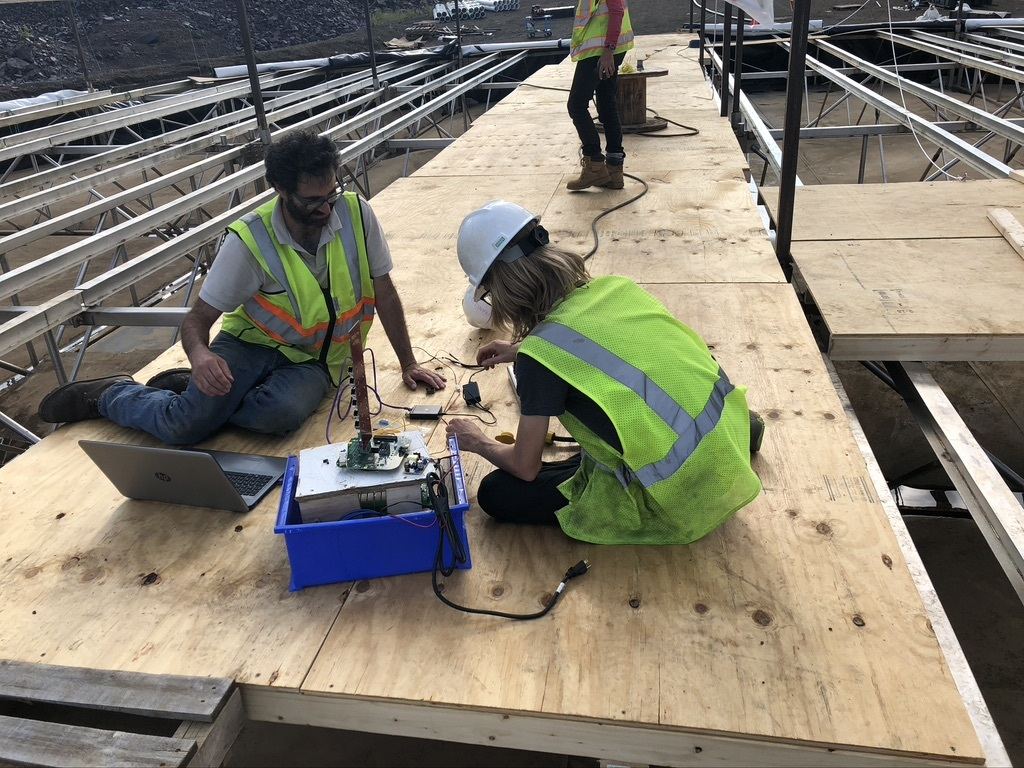
\includegraphics[height=6.5cm]{diagrams/4-chips/work1.jpeg}%
    }
    \quad
    \subcaptionbox{Making floatation}{%
        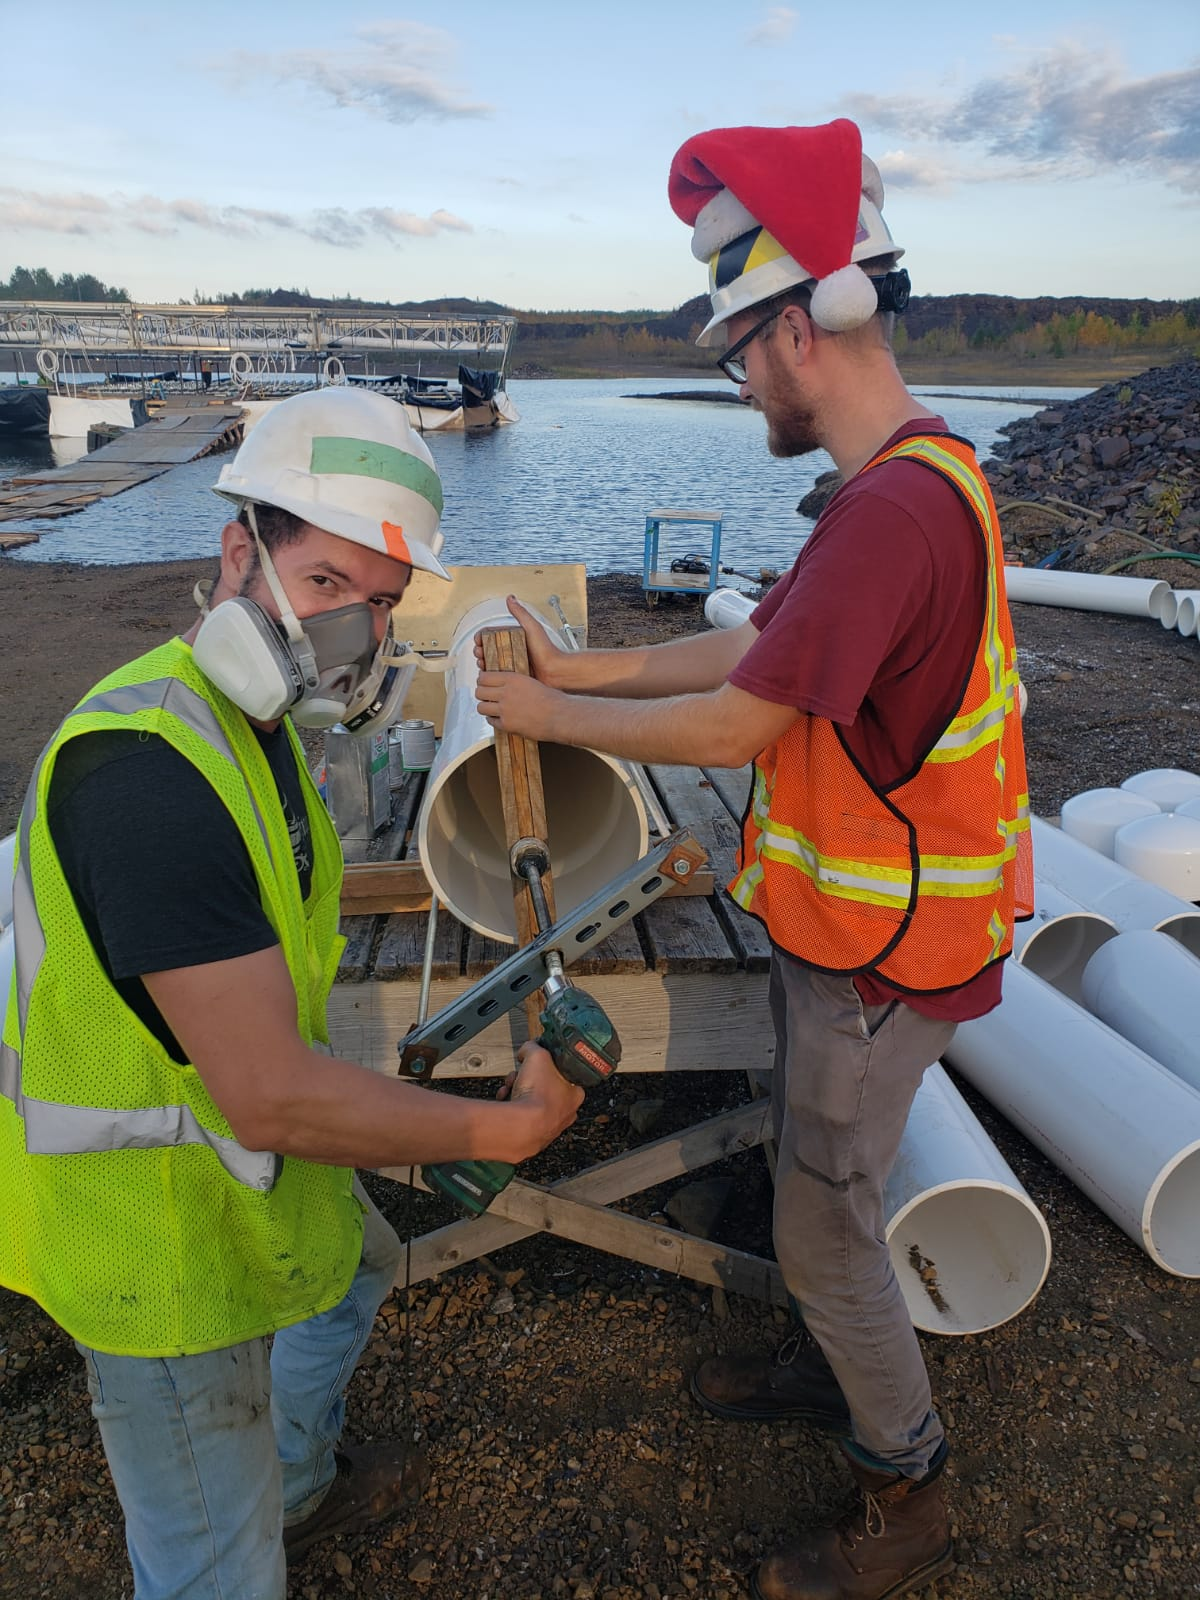
\includegraphics[height=6.5cm]{diagrams/4-chips/work3.jpg}%
    }
    \caption[afaga]
    {Construction work on the \chipsfive detector.}
    \label{fig:work1}
\end{figure}

\begin{figure} % WORK DIAGRAM %
    \centering
    \subcaptionbox{Installing a POM}{%
        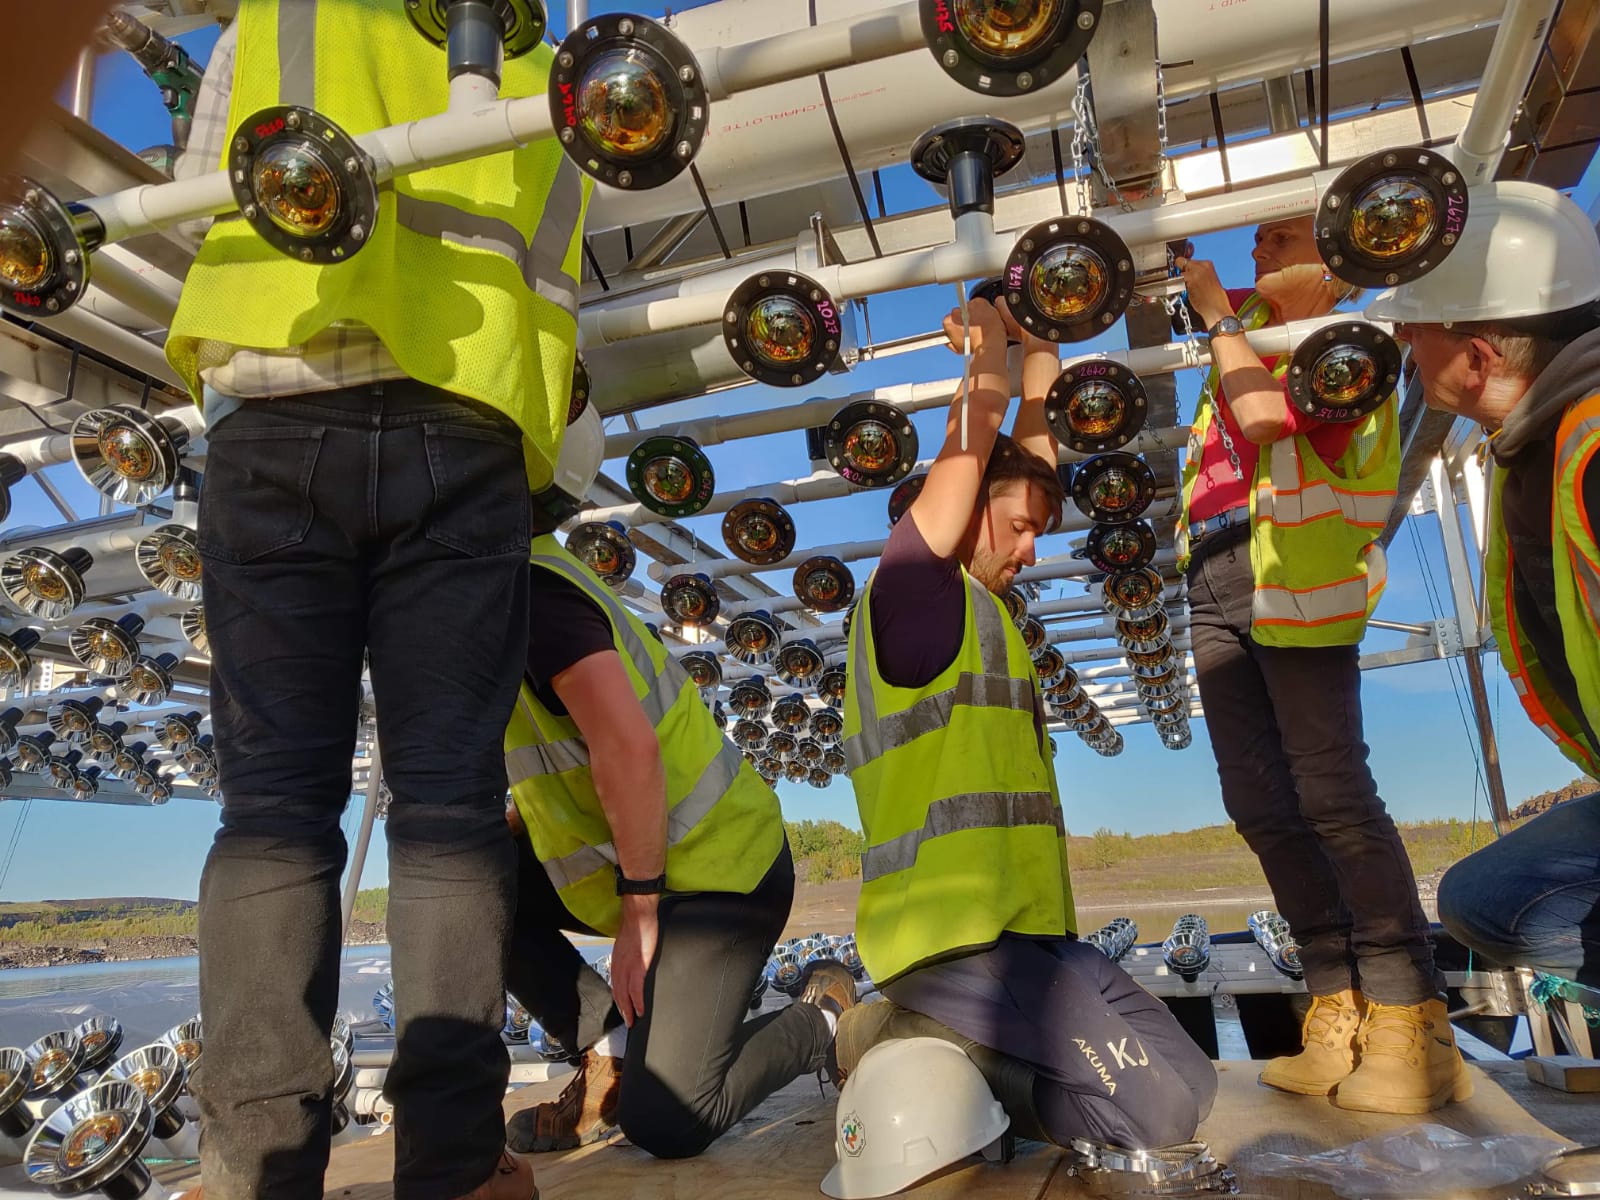
\includegraphics[height=5.6cm]{diagrams/4-chips/work4.jpg}%
    }
    \quad
    \subcaptionbox{Fixing a POM}{%
        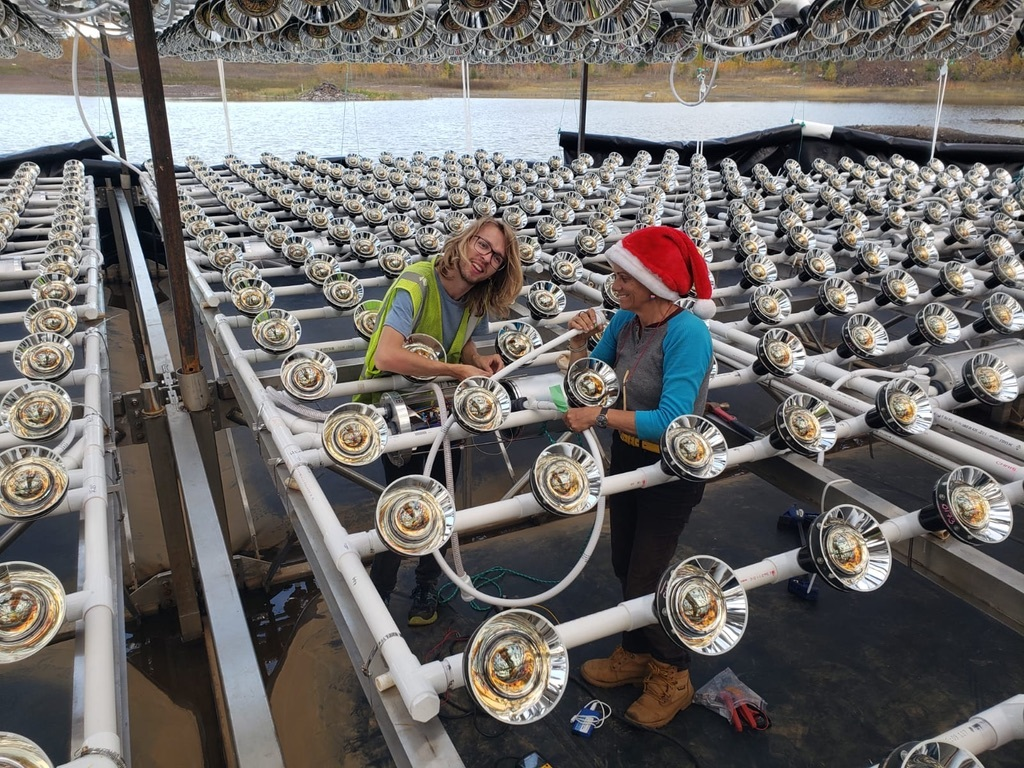
\includegraphics[height=5.6cm]{diagrams/4-chips/work2.jpeg}%
    }
    \caption[afaga]
    {Construction work on the \chipsfive detector.}
    \label{fig:work2}
\end{figure}

\begin{figure} % PANORAMA DIAGRAM %
    \includegraphics[width=\textwidth]{diagrams/4-chips/pan_1.jpeg}
    \caption[Panorama of the inside of \chipsfive just before deployment.]
    {Panorama of the inside of \chipsfive just before deployment. The six deployed Madison POMs
        are visible in the foreground on the bottom endcap. Additionally, the flexible tube
        manifolds can be seen connecting each POM to the higher level DAQ electronics.}
    \label{fig:pan_1}
\end{figure}

\section{Event generation and detector simulation} %%%%%%%%%%%%%%%%%%%%%%%%%%%%%%%%%%%%%%%%%%%%%%%
\label{sec:chips_monte_carlo} %%%%%%%%%%%%%%%%%%%%%%%%%%%%%%%%%%%%%%%%%%%%%%%%%%%%%%%%%%%%%%%%%%%%

Monte carlo event generation and detector simulation methods are an indispensable tool within high
energy particle physics. This is particularly true during the design and prototyping phase of an
experimental project when no real world data is available, as is the case with \chips. By matching
the observables of a real world detector as closely as possible, these methods allow for the
optimisation of designs, the testing of reconstruction techniques and the study of physics
sensitivities. Here, the beam and cosmic event generation procedures and a description of the
detector simulation used by \chips are described. All are used extensively for work presented in
later chapters of this thesis.

\subsection{Beam event generation} %%%%%%%%%%%%%%%%%%%%%%%%%%%%%%%%%%%%%%%%%%%%%%%%%%%%%%%%%%%%%%%
\label{sec:chips_monte_carlo_beam} %%%%%%%%%%%%%%%%%%%%%%%%%%%%%%%%%%%%%%%%%%%%%%%%%%%%%%%%%%%%%%%

The expected flux of beam neutrinos at the \chipsfive detector location is generated using the
existing beam simulation written for the \numi experiments, and shown in Fig.~\ref{fig:flux}. As
the $\nu_{\tau}$ component is negligible, it is not predicted by the beam simulation and ignored.
Using the generated fluxes as input the GENIE neutrino event generator (version
3.0.6)~\cite{andreopoulos2009, andreopoulos2015} is used to generate beam neutrino events. Default
cross-sections on water provided by GENIE are used. All initial, intermediate, and final state
particle tracks for each event are stored as output in a NUANCE formatted file for use in the
detector simulation. Note that unoscillated fluxes are used such that analyses samples must be
weighted to match the desired oscillated neutrino composition.

\begin{figure} % CHIPS FLUX DIAGRAM %
    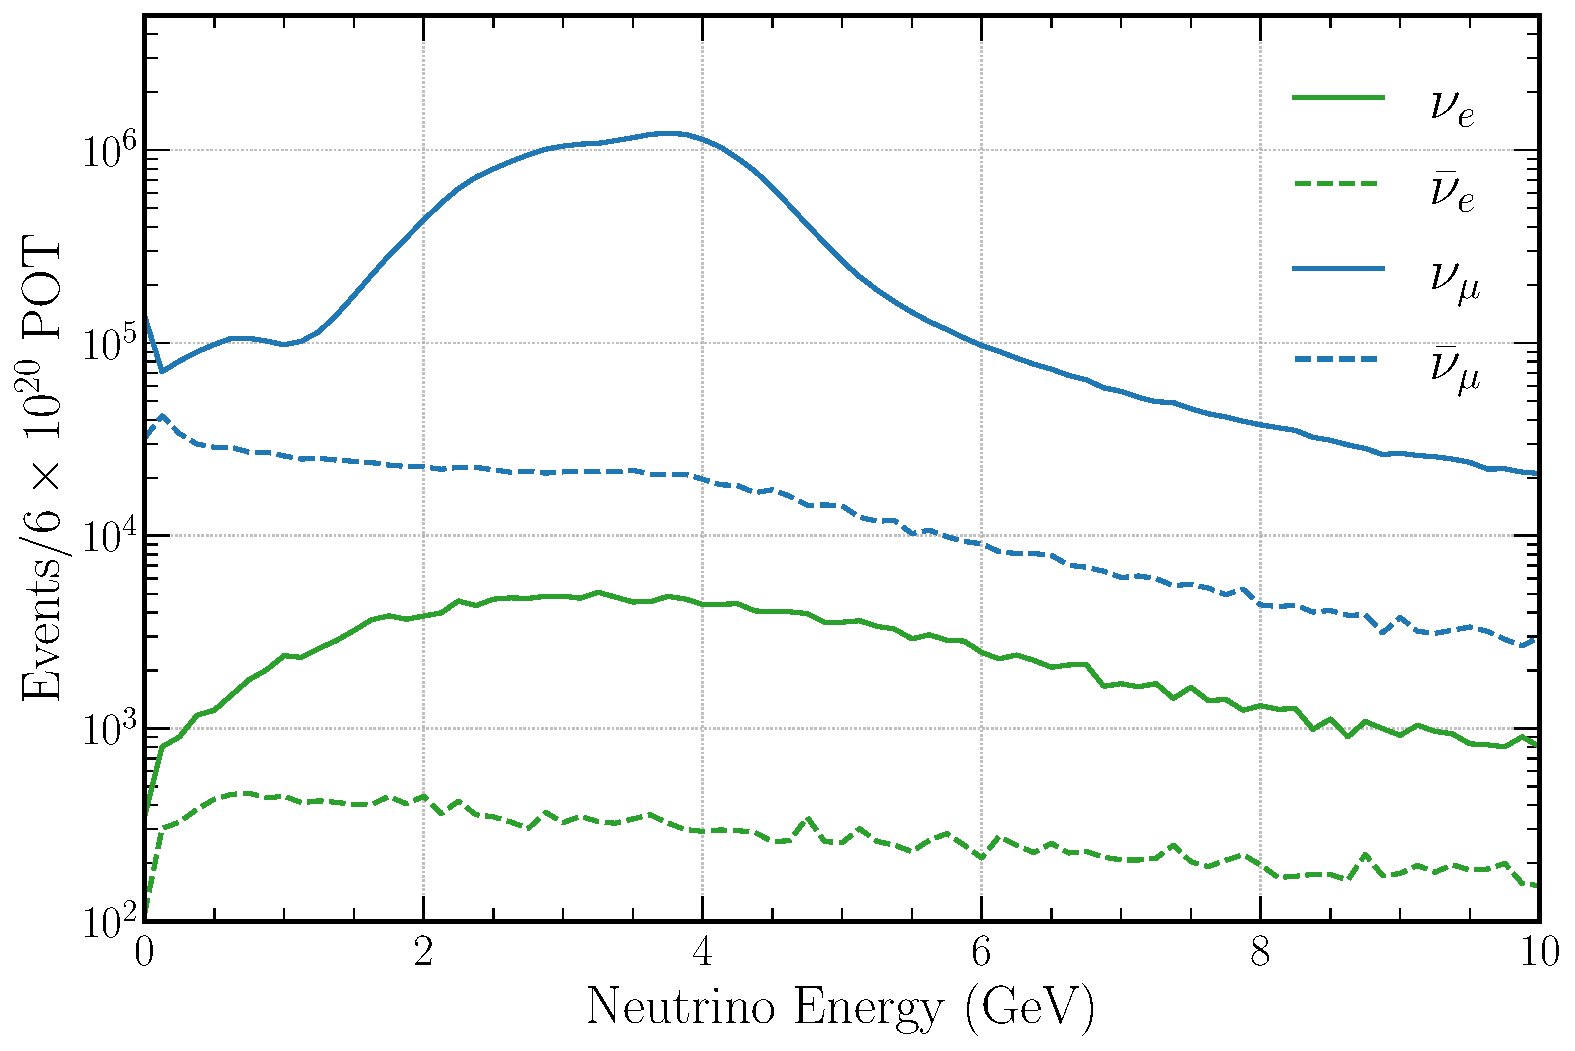
\includegraphics[width=0.8\textwidth]{diagrams/4-chips/flux.pdf}
    \caption[\numi neutrino flux at CHIPS.]
    {The neutrino mode (forward horn current) \numi beam neutrino energy spectrum at the
        \chipsfive detector module location. Shown are the separate contributions from the
        different neutrino types and signs. No cross-sections or oscillations have been applied.}
    \label{fig:flux}
\end{figure}

\subsection{Cosmic event generation} %%%%%%%%%%%%%%%%%%%%%%%%%%%%%%%%%%%%%%%%%%%%%%%%%%%%%%%%%%%%%
\label{sec:chips_monte_carlo_cosmic} %%%%%%%%%%%%%%%%%%%%%%%%%%%%%%%%%%%%%%%%%%%%%%%%%%%%%%%%%%%%%

The Cosmic-Ray Shower Library (CRY)~\cite{hagmann2012_1, hagmann2012_2} is used for cosmic ray
event generation. Both the solar cycle and Earth's geomagnetic field are taken into account, with
the \chipsfive latitude and deployment date (1st November 2019) used as input. Single muons are
generated at sea level by CRY within a \unit{1}{\mathrm{km}}$\times$\unit{1}{\mathrm{km}} area,
with the detector at it's centre. Note that only single muon events (the dominant cosmic
component) are considered for simplicity.

Assuming a \chipsfive overburden of \unit{50}{\mathrm{m}} and a \unit{2.2}{\MeV/\mathrm{cm}^{2}}
muon energy loss in water as suggested by Ref.~\cite{klimushin2001} the muon parameters are
updated to estimate their values \unit{1}{\mathrm{m}} above the top of the detector. All muons
whose path does not cross the detector volume or do not have sufficient energy to reach the
detector are discarded~\cite{chipsgen2020}. All accepted muon tracks are stored as output in a
NUANCE formatted file for use in the detector simulation.

In order to use generated cosmic events in analysis, studies have looked at the likely cosmic rate
for \chips detector modules at different water overburden depths~\cite{son2013}. In this work, the
fits shown in Fig.~\ref{fig:cosmic_rate} for a cylindrical detector of both height and diameter
\unit{24}{\mathrm{m}} are used to estimate a \chipsfive cosmic muon rate of
\unit{11.8}{\mathrm{KHz}} with \unit{50}{\mathrm{m}} of overburden.

Given the \unit{10}{\mu\mathrm{s}} long \numi beam spill occurring every \unit{1.33}{\mathrm{s}}
this gives an in spill cosmic rate of $\sim2.1$ million events per year and an in spill occupancy
of 9\%. Considering a typical event takes $\sim$\unit{100}{\mathrm{ns}} to unfold, there is
approximately a 0.3\% chance that any beam event overlaps with a cosmic muon. This low coincidence
shows just how powerful a short beam spill can be at reducing the significant cosmic background.

\begin{figure} % COSMIC RATE DIAGRAM %
    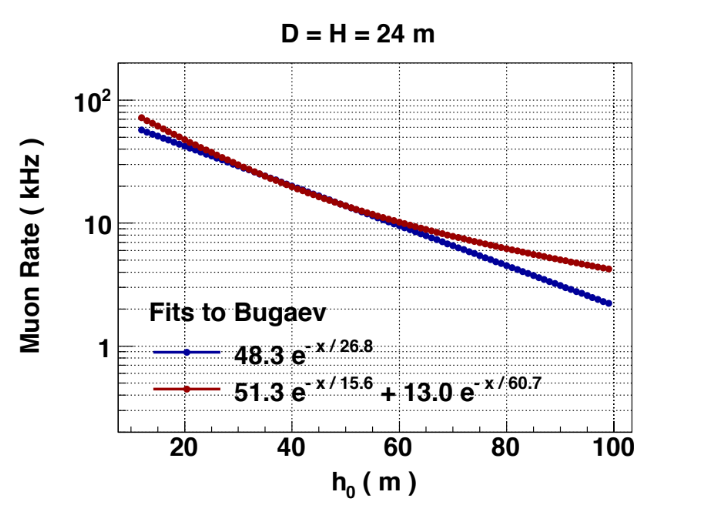
\includegraphics[width=0.6\textwidth]{diagrams/4-chips/cosmic_rate.png}
    \caption[Expected \chipsfive cosmic muon rate as a function of depth.]
    {Expected cosmic muon rate as a function of water overburden depth for a \unit{24}{\mathrm{m}}
        high and \unit{24}{\mathrm{m}} wide \chips detector module. Shown are fits made to the
        work originally conducted in Ref.~\cite{bugaev1998}. Figure taken from
        Ref.~\cite{son2013}.}
    \label{fig:cosmic_rate}
\end{figure}

\subsection{Detector simulation} %%%%%%%%%%%%%%%%%%%%%%%%%%%%%%%%%%%%%%%%%%%%%%%%%%%%%%%%%%%%%%%%%
\label{sec:chips_monte_carlo_sim} %%%%%%%%%%%%%%%%%%%%%%%%%%%%%%%%%%%%%%%%%%%%%%%%%%%%%%%%%%%%%%%%

The detector simulation uses the WCSim water Cherenkov simulation package~\cite{wcsim2020} built
on top of the Geant4 simulation framework~\cite{agostinelli2003, allison2006, Allison2016}.
Originally developed to simulate possible water Cherenkov detectors in the LBNE beam (now LBNF),
WCSim is now used more widely in the field. WCSim has been heavily modified for the \chips project
to allow for generic water Cherenkov detector geometries to be easily loaded at runtime via a
series of simple XML configuration files. These changes allow for a broad range of detector
geometries to be quickly considered without recompilation of the code.

To represent \chips detector modules, the simulation builds an n-sided, regular polygonal prism
consisting of two endcaps separated by a barrel. The prism is filled with water and lined with a
low reflectivity \emph{blacksheet}. The geometry is separated into \emph{regions} within both the
barrel and endcaps, defined either by a list of barrel sides or an opening angle respectively.
Each region is filled with a unique base unit of geometry known as the \emph{unit cell} as shown
in Fig.~\ref{fig:sim_geom}.

The unit cell defines a pattern of any number of PMTs, as well as their relative positions and in
which direction they face. The final geometry is built by tiling each of the defined regions with
their respective unit cell scaled to match the required regional photocathode coverage. Note that
although exact PMT positions are not used in this procedure, a given configuration will always
generate the same geometry (it is deterministic). In this work the \chipsfive geometry is
generated with 28 sides and regions matching the angles and photocathode coverage detailed in
Section.~\ref{sec:chips_detector_instrumentation}.

\begin{figure} % SIMULATION GEOM DIAGRAM %
    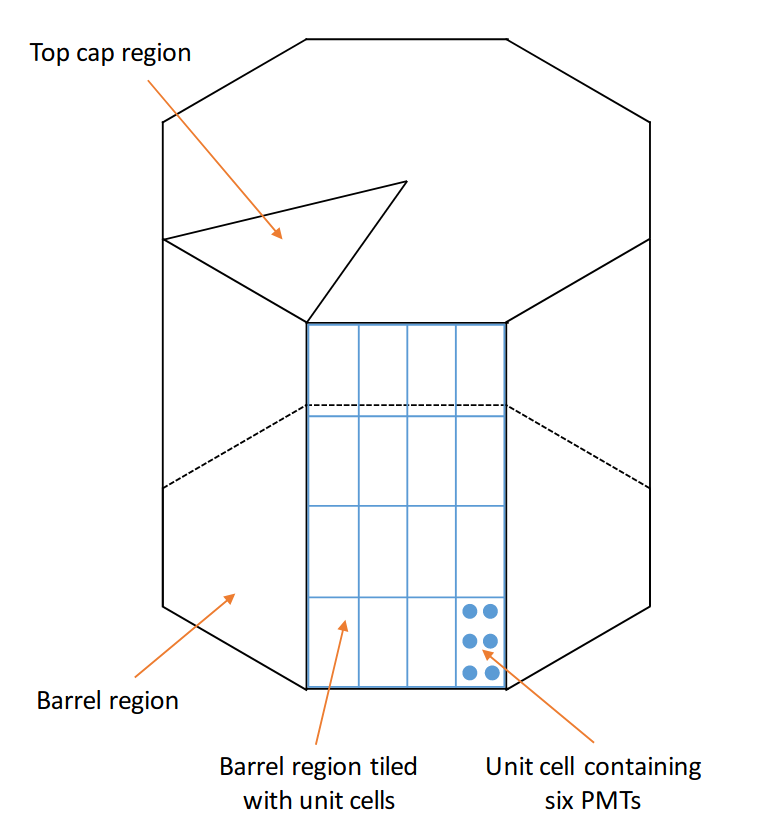
\includegraphics[width=0.6\textwidth]{diagrams/4-chips/sim_geom.png}
    \caption[Illustrative diagram of a WCSim detector geometry.]
    {Illustrative diagram of a WCSim detector geometry, showing the shape, endcap and barrel
        regions, tiled unit cells and PMTs within a unit cell. Figure taken from
        Ref.~\cite{blake2016}.}
    \label{fig:sim_geom}
\end{figure}

The geometry shape, regions, and unit cells are defined in a configuration file. Additionally, a
file for PMT definitions containing their shape, time resolution, and quantum efficiency is
defined. Light cones are described by a list of radial profile points in a further file. Although
the underlying Geant4 material properties are mostly hardcoded (taken from the Super-Kamiokande
simulation) they can be scaled by values within yet another configuration file. This file controls
the water absorption and scattering (Rayleigh and Mie) lengths, and both the blacksheet and PMT
glass reflectivity. In this work an attenuation length of \unit{50}{\mathrm{m}} at
\unit{405}{\mathrm{nm}} is used with negligible scattering, the blacksheet reflectivity is set to
be 4\% and the PMT glass reflectivity 24\%.

A veto volume can also be defined. The veto is built as either a concentric shell around the whole
inner volume with a given thickness or solely above the top-cap with a given height. Any PMTs
defined as facing outwards within a unit cell look into the veto volume instead of the inner
volume. In this work the \chipsfive geometry is given a top-cap veto of height
\unit{1.3}{\mathrm{m}}.

Once the full generation of the runtime Geant4 geometry is complete, the final state tracks for
each successive event to be simulated are loaded from either the beam or cosmic event generator
NUANCE files. Beam event vertices are randomly placed within the inner detector volume, while
cosmic vertices are kept at \unit{1}{\mathrm{m}} above the detector volume. WCSim then simulates
the passage of all particles through the detector materials, additionally interactions, decays,
and Cherenkov emission are also considered.

Whenever a photon is calculated to have hit the photocathode of a PMT an angular dependent
acceptance efficiency is applied to see if it is recorded. If accepted all hits within
\unit{200}{\mathrm{ns}} windows are grouped together to form a single recorded hit, with the
smeared first hit time used as the recorded time. A method similar to that used in the
Super-Kamiokande simulation determines the total output charged of the hit given the number of
incident photons. A single photoelectron charge distribution is probed for each photon and the
combined sum returned. By sampling this procedure multiple times, the output charge probability
distribution given the number of incident photons is shown in Fig.~\ref{fig:digitisation}. The
figure also shows the reverse \emph{likelihood} function (lower is more likely) of an actual
number of incident photons given a measured digitised charge.

\begin{figure} % DIGI DIAGRAM %
    \centering
    \subcaptionbox{\label{fig:digi_method}}{%
        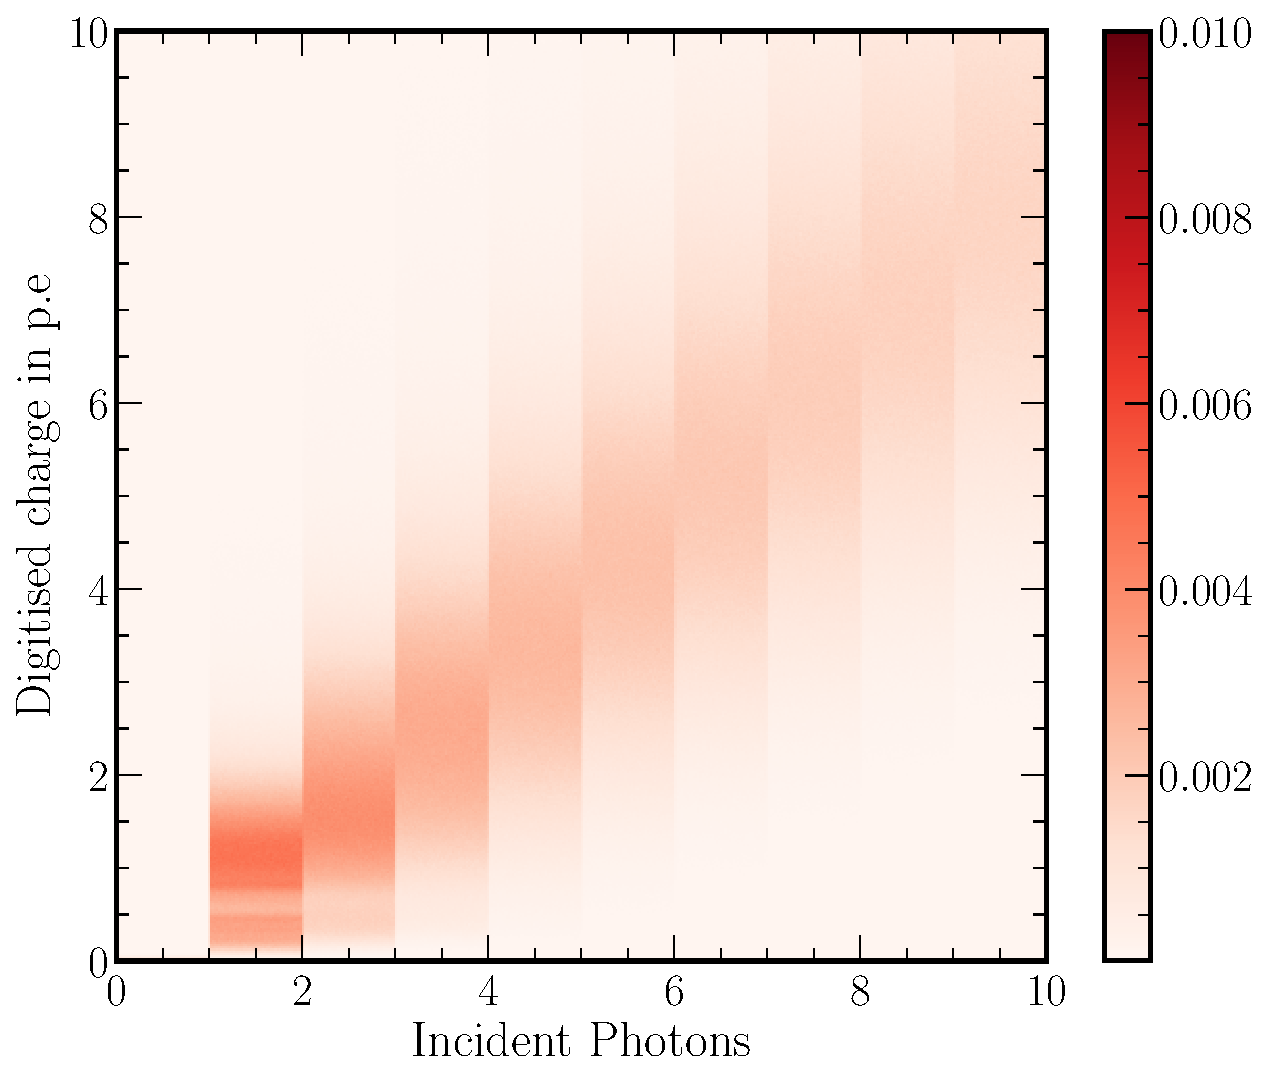
\includegraphics[height=6cm]{diagrams/4-chips/digi_method.pdf}%
    }
    \quad
    \subcaptionbox{\label{fig:digi_likelihood}}{%
        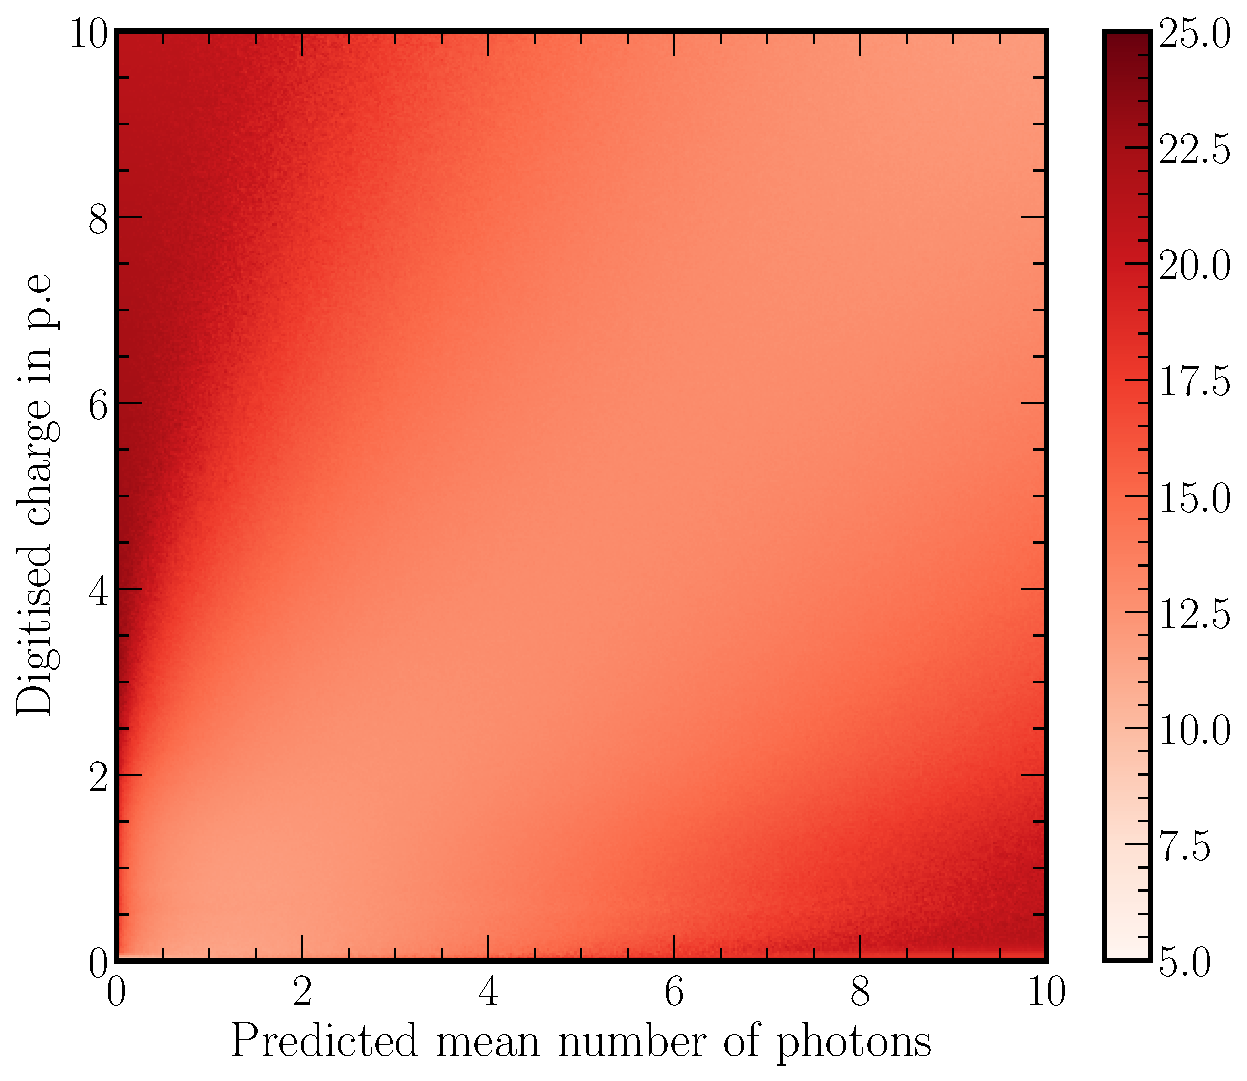
\includegraphics[height=6cm]{diagrams/4-chips/digi_likelihood.pdf}%
    }
    \caption[Detector simulation PMT digitisation function.]
    {The detector simulation digitisation probability function (a) used for the Nikhef

        (a) Digitisation probability function used within the simulation to convert incident
        photons to a measured digitised charge. (b) Likelihood of a measured digitised charge
        being caused by a number of photons incident on a PMT.}
    \label{fig:digitisation}
\end{figure}

All fully simulated PMT hits for each event are stored in an output ROOT file. Additionally,
important truth information about the neutrino interaction and keys tracks is included. A full
event takes approximately \unit{3}{\mathrm{seconds}} to simulate on a standard batch farm
computing node. An example output event display for a CC $\nu_{\mu}$ event is shown in
Fig.~\ref{fig:sim_event}.

\begin{figure} % SIMULATED EVENT DISPLAY DIAGRAM %
    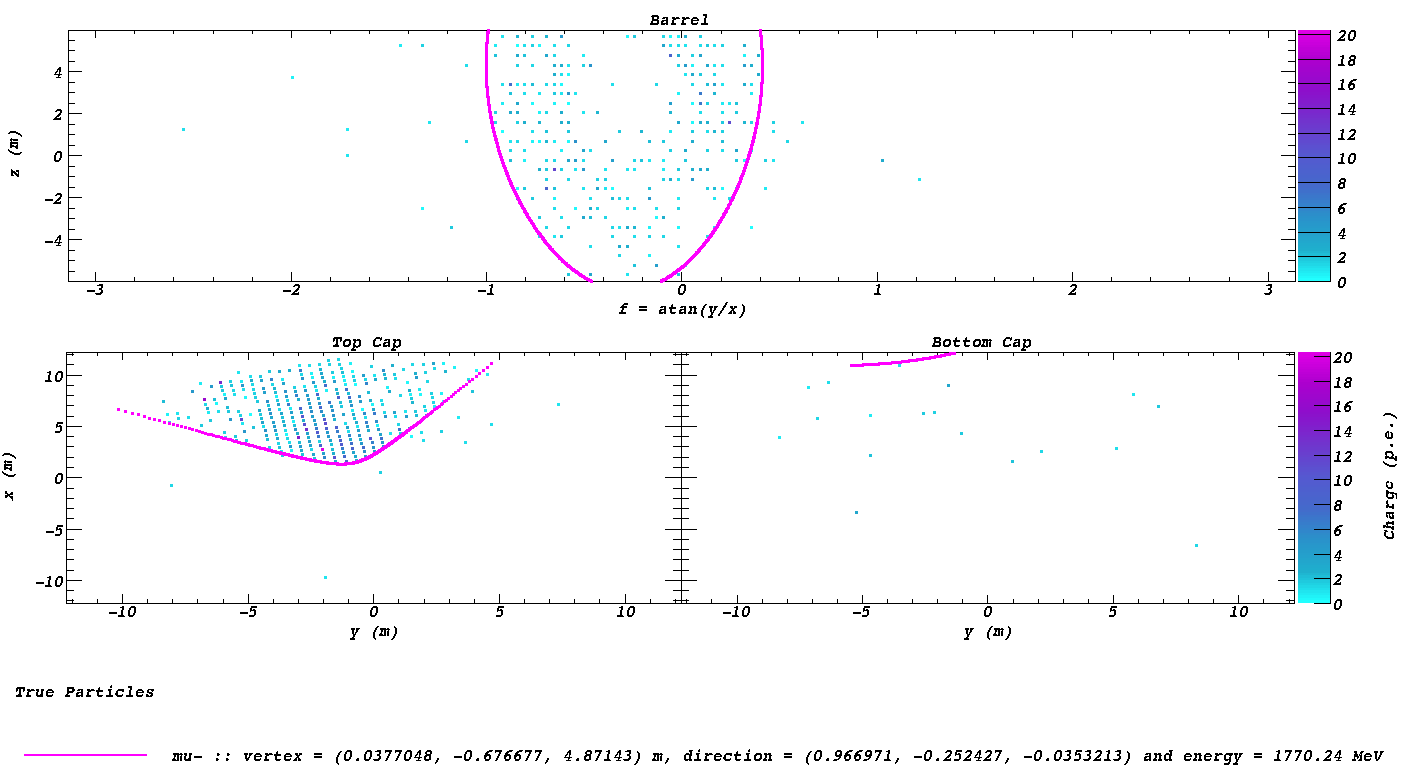
\includegraphics[width=\textwidth]{diagrams/4-chips/sim_event.png}
    \caption[sim event short]
    {Event display of a simulated CC $\nu_{\mu}$ quasi-elastic event with a single muon in the
        final state of energy \unit{1.77}{\GeV}. The display shows both the unrolled barrel of the
        \chipsfive detector as well the two endcaps. Every coloured entry represents a hit PMT
        with the color indicating the total photoelectrons (charge) collected. The pink ring is a
        projection of the true Cherenkov light cone associated with the muon track from the
        interaction vertex.}
    \label{fig:sim_event}
\end{figure}
